% !TeX program = pdflatex
% !TeX spellcheck = en_US
% !TeX encoding = UTF-8

% update
% v.1.2 - 2018-10-15
% - Felix: use Bibtex instead of Biblatex
% v1.10 - 2017-05-30
% - Erik: Refactor the file structure of the front pages
% - Erik: Fix double bibliography entry
% v1.9 - 2017-02-03
% - Dirk: fixed warning: Underfull \hbox (badness 10000) in paragraph main.tex
% - Dirk: fixed warning: "Data encoding is UTF8" -> style.tex 0.1.8
% v1.8 - 2017-02-02
% - Dirk: replaced titlesec package by KOMA-script commands.-> style.tex v0.1.7
% v1.7 - 2014-11-18
% - bib fixes: now using biber instead of bibtex (thanks felix)
% - compile now with pdflatex -> biber -> pdflatex
% v1.6 - 2013-05-13
% - bibliography headers fixed - thanx lorenz lehmann
% - high quality titlepage - thanx thomas graf
% - removed separation of online and offline references -> style 1.4a
% v1.5 - 2013-01-16

\documentclass[twoside,11pt,titlepage,a4paper,english,bibliography=totocnumbered,listof=numbered]{scrbook}
%
% Template Style
% =========================================================================
% = SNET THESIS TEMPLATE STYLE
% =========================================================================

% http://www.snet.tu-berlin.de
% ------------------------
% Adapted version from http://hci.rwth-aachen.de/karrer_thesistemplate (Thorsten Karrer)
% Further adaptions for http://www.elearn.rwth-aachen.de (Sascha Hoellger)
% Further adaptions for SNET @ TU Berlin by Sebastian Göndör (sebastian.goendoer@tu-berlin.de)


% =========================================================================
% = CHANGELOG
% =========================================================================
% [0.1.9]
% - Fixed styling for chapters and toc using Komascript
% - Remove double bibliography TOC entry
%
% [0.1.8]
% - fixed "warning UFT8 is used". biblatex requires ascii encoding; by Dirk
%
% [0.1.7]
% replaced "Titelsec" commands (and whole package) by appropriate KOMA-Script commands; by Dirk
%
% [0.1.6]
% replaced deprecated \rm commands with \rmfamily commands; by Dirk
%
% [0.1.4b]
% backend=biber added in line 139
%
% [0.1.4a]
% title page: image logo sizes and margins adjusted to printable area
% removed separation of online and offline references
%
% [0.1.3]
% wider text body
% added "school" to the titlepage
% paragraph indents
% correctly placed footnote graphics
%
% [0.1.2]
% new titlepage
% some minor fixes
%
% [0.1.1]
% changed titlepage logo
% added listoffigures and listoftables
% excluded abstract from toc
% no (roman) numbering for frontmatter
%
% [0.1]
% adapted version 0.991b from sascha hoellger @ rwth aachen


% =========================================================================
% = MISC
% =========================================================================

\usepackage{a4wide}					%
\usepackage{verbatim}				%
\usepackage[toc,page]{appendix}			%
\usepackage[withpage]{acronym}			%
\usepackage{amsthm}				% Definitions


% =========================================================================
% = COLORS
% =========================================================================

\usepackage{xcolor}					% Colors
\definecolor{LightBlue}{rgb}{0.55,0.55,1}
\definecolor{DarkBlue}{rgb}{0.2,0.2,0.5}
\definecolor{DarkRed}{rgb}{0.71,0.12,0.07}

% =========================================================================
% = PAGE LAYOUT
% =========================================================================

\usepackage{geometry}
\geometry{inner=3cm, outer=2cm, bottom=4cm}

\newcommand{\setwidesite}				% changes the geometry to have less margin
{
	\fancyhfoffset[LE,RO]{0cm}
	\fancyheadoffset[LO,RE]{0cm}
	\fancyfootoffset[RE]{2cm}
	\newgeometry{inner=2cm, outer=2cm, bottom=4cm}
}

\usepackage{style/noindent}				%do not indent at new paragraphs but add a vertical offset

\setlength{\parindent}{4mm}
\setlength{\parskip}{1.5mm }


% =========================================================================
% = TYPESETTING
% =========================================================================

\usepackage[hyphens]{url}				% url
\usepackage{hyphenat}				% hyphenation. use \hyphenation{}

\righthyphenmin=5
\lefthyphenmin=5


% =========================================================================
% = TABLE OF CONTENTS
% =========================================================================

\setcounter{secnumdepth}{4}
\setcounter{tocdepth}{3}

\addtokomafont{disposition}{\rmfamily}


% =========================================================================
% = FONTS
% =========================================================================

\usepackage{mathpazo}
\usepackage[scaled=.95]{helvet}
\usepackage{courier}


% =========================================================================
% = SYMBOLS
% =========================================================================

%\usepackage{gensymb}
\usepackage{textcomp} 				% for \textmu (non-italic $\mu$)
\makeatletter						% this makes "@" a regular letter


% =========================================================================
% = TABLES
% =========================================================================

\usepackage{tabularx}
\usepackage{booktabs}
\usepackage{multirow}
\usepackage{longtable}				% tables spanning over more than one page

%%\setlength{\fboxsep}{0mm}			% spacing between \fbox border and content

\usepackage{amsmath}				% math fonts
\usepackage{amssymb}				% math symbols
\usepackage{setspace}				% line spacing


% =========================================================================
% = BIBILOGRAPHY
% =========================================================================

% 2018-10-16 - changed to use Bibtex instead

%\usepackage[style=numeric,natbib=true,backend=biber]{biblatex}

% apparently no effect?
%\renewcommand{\bibsetup}{
%	\markboth{
%		\MakeUppercase{Bibliography}
%	}{}
%}

%\ifdefined\bibheadingonline
%  \defbibheading{online}{\section*{\bibheadingonline}}
%\else
%  \defbibheading{online}{\section*{Online References}}
%\fi
%\ifdefined\bibheadingoffline
%  \defbibheading{offline}{\section*{\bibheadingoffline}}
%\else
%  \defbibheading{offline}{\section*{Printed References}}
%\fi
%
%\defbibfilter{online}{%
%  \( \type{online} \)}
%
%\defbibfilter{offline}{%
%  \( \not \type{online} \)}
%
%\bibliography{Bibliography}


% =========================================================================
% = LANGUAGE & ENCODING
% =========================================================================

\usepackage[english]{babel}				% \usepackage[ngerman]{babel}

\selectlanguage{english}				% \selectlanguage{ngerman}

\usepackage[T1]{fontenc}
\usepackage[utf8]{inputenc}				% can use native umlauts

% \usepackage[babel,german=quotes]{csquotes}	% provides \enquote{Blupp} => "`Blupp"'
\usepackage[babel,english=american]{csquotes}	% provides \enquote{Blupp} => "`Blupp"'

%\SetCiteCommand{\parencite}			% Changed for biblatex

\usepackage{units}					% unified way of setting values with units

\usepackage{appendix}


% =========================================================================
% = CODE LISTINGS
% =========================================================================

\usepackage{listings}

% Listings Styles from Max

\definecolor{violet}{cmyk}{0.45,0.97,0.27,0.21}
\definecolor{lstblue}{cmyk}{1,0.80,0,0}
\definecolor{lstgreen}{cmyk}{0.71,0.21,0.65,0.22}
\definecolor{bluegrey}{cmyk}{0.56,0.24,0.11,0.05}
\definecolor{javadoc}{cmyk}{0.88,0.59,0,0}
\definecolor{lstgrey}{cmyk}{0.55,0.44,0.42,0.32}

\lstdefinelanguage{SQL}{
     keywords={},
     keywordstyle=\color{bluegrey}\bfseries,
     morekeywords=[2]{CREATE,TABLE,IF,NOT,EXISTS,NULL,SET,DEFAULT,PRIMARY,KEY,COLLATE,CHARACTER,AUTO_INCREMENT,ENGINE,CHARSET},
     keywordstyle={[2]\color{violet}\bfseries},
     otherkeywords={int,varchar,double,text,tinyint},
     sensitive=false,
     morecomment=[l][\color{lstgreen}]{//},
     morecomment=[s][\color{lstgreen}]{/*}{*/},
     morecomment=[s][\color{javadoc}]{/**}{*/},
     morestring=[b]',
     morestring=[b]"
  }
\lstdefinelanguage{PHP}{
     keywords={},
     keywordstyle=\color{bluegrey}\bfseries,
     morekeywords=[2]{static,function,if,return,pow,sin,cos,asin,min,sqrt,int},
     keywordstyle={[2]\color{violet}\bfseries},
     otherkeywords={@param, @returns, @author, @type, @link, @see},
     sensitive=false,
     morecomment=[l][\color{lstgreen}]{//},
     morecomment=[s][\color{lstgreen}]{/*}{*/},
     morecomment=[s][\color{javadoc}]{/**}{*/},
     morestring=[b]',
     morestring=[b]"
  }
\lstdefinelanguage{JavaScript}{
     keywords={},
     keywordstyle=\color{bluegrey}\bfseries,
     morekeywords=[2]{attributes, class, classend, do, empty, endif, endwhile, fail, function, functionend, if, implements, in, inherit, inout, not, of, operations, out, return, set, then, types, while, use},
     keywordstyle={[2]\color{violet}\bfseries},
     otherkeywords={@param, @returns, @author, @type, @link, @see},
     sensitive=false,
     morecomment=[l][\color{lstgreen}]{//},
     morecomment=[s][\color{lstgreen}]{/*}{*/},
     morecomment=[s][\color{javadoc}]{/**}{*/},
     morestring=[b]',
     morestring=[b]"
  }
\lstdefinelanguage{Java}{
     keywords={},
     keywordstyle=\color{bluegrey}\bfseries,
     morekeywords=[2]{abstract,boolean,break,byte,case,catch,char,class,
      const,continue,default,do,double,else,extends,false,final,
      finally,float,for,goto,if,implements,import,instanceof,int,
      interface,label,long,native,new,null,package,private,protected,
      public,return,short,static,super,switch,synchronized,this,throw,
      throws,transient,true,try,void,volatile,while},
     keywordstyle={[2]\color{violet}\bfseries},
     morekeywords=[3]{@SuppressWarnings, @Capability, @Override},
     keywordstyle={[3]\color{lstgrey}},
     otherkeywords={@param, @return, @returns, @author, @link, @see},
     sensitive,
     morecomment=[l]//,
     morecomment=[s]{/*}{*/},
     morecomment=[s][\color{javadoc}]{/**}{*/},
     morestring=[b]",
     morestring=[b]',
  }[keywords,comments,strings]

% some listings styles from Gregor Aisch
% http://vis4.net/blog/2009/09/noch-mehr-sprach-definitionen-fuer-latex-listings/

\lstdefinelanguage{HTML5} {morekeywords={a, abbr, address, area, article, aside, audio, b, base, bb, bdo, blockquote,  body, br, button, canvas, caption, cite, code, col, colgroup, command, datagrid, datalist, dd, del, details, dialog, dfn, div, dl, dt, em, embed, eventsource, fieldset, figure, footer,  form,  h1, h2,  h3,  h4, h5,  h6,  head,  header,  hr, html,  i, iframe,  img,  input,  ins, kbd,  label,  legend,  li,  link,  mark,  map,  menu,  meta,  meter,  nav,  noscript,  object,  ol,  optgroup,  option,  output,  p,  param,  pre,  progress,  q,  ruby,  rp,  rt,  samp,  script,  section,  select,  small,  source,  span,  strong,  style,  sub,  sup,  table,  tbody,  td,  textarea,  tfoot,  th,  thead,  time,  title,  tr,  ul,  var,  video},
sensitive=false, morecomment=[s]{<!--}{-->}, morestring=[b]", morestring=[d]'}

\lstdefinelanguage{CSS} {morekeywords={azimuth,  background-attachment,  background-color,  background-image,  background-position,  background-repeat,  background,  border-collapse,  border-color,  border-spacing,  border-style,  border-top, border-right, border-bottom, border-left,  border-top-color, border-right-color, border-bottom-color, border-left-color,  border-top-style, border-right-style, border-bottom-style, border-left-style,  border-top-width, border-right-width, border-bottom-width, border-left-width,  border-width,  border,  bottom,  caption-side,  clear,  clip,  color,  content,  counter-increment,  counter-reset,  cue-after,  cue-before,  cue,  cursor,  direction,  display,  elevation,  empty-cells,  float,  font-family,  font-size,  font-style,  font-variant,  font-weight,  font,  height,  left,  letter-spacing,  line-height,  list-style-image,  list-style-position,  list-style-type,  list-style,  margin-right, margin-left,  margin-top, margin-bottom,  margin,  max-height,  max-width,  min-height,  min-width,  orphans,  outline-color,  outline-style,  outline-width,  outline,  overflow,  padding-top, padding-right, padding-bottom, padding-left,  padding,  page-break-after,  page-break-before,  page-break-inside,  pause-after,  pause-before,  pause,  pitch-range,  pitch,  play-during,  position,  quotes,  richness,  right,  speak-header,  speak-numeral,  speak-punctuation,  speak,  speech-rate,  stress,  table-layout,  text-align,  text-decoration,  text-indent,  text-transform,  top,  unicode-bidi,  vertical-align,  visibility,  voice-family,  volume,  white-space,  widows,  width,  word-spacing,  z-index},
sensitive=false, morecomment=[s]{/*}{*/}, morestring=[b]", morestring=[d]'}

\lstdefinelanguage{JavaFX} {morekeywords={abstract, after, and, as, assert, at, attribute, before, bind, bound, break, catch, class, continue, def, delete, else, exclusive, extends, false, finally, first, for, from, function, if, import, indexof, in, init, insert, instanceof, into, inverse, last, lazy, mixin, mod, new, not, null, on, or, override, package, postinit, private, protected, public-init, public, public-read, replace, return, reverse, sizeof, static, step, super, then, this, throw, trigger, true, try, tween, typeof, var, where, while, with },
sensitive=false, morecomment=[l]{//}, morecomment=[s]{/*}{*/}, morestring=[b]", morestring=[d]'}

\lstdefinelanguage{MXML} {morekeywords={mx:Accordion, mx:Box, mx:Canvas, mx:ControlBar, mx:DividedBox, mx:Form, mx:FormHeading, mx:FormItem, mx:Grid, mx:GridItem, mx:GridRow, mx:HBox, mx:HDividedBox, mx:LinkBar, mx:Panel, mx:TabBar, mx:TabNavigator, mx:Tile, mx:TitleWindow, mx:VBox, mx:VDividedBox, mx:ViewStack, mx:Button, mx:CheckBox, mx:ComboBase, mx:ComboBox, mx:DataGrid, mx:DateChooser, mx:DateField, mx:HRule, mx:Image, mx:Label, mx:Link, mx:List, mx:Loader, mx:MediaController, mx:MediaDisplay, mx:MediaPlayback, mx:MenuBar, mx:NumericStepper, mx:ProgressBar, mx:RadioButton, mx:RadioButtonGroup, mx:Spacer, mx:Text, mx:TextArea, mx:TextInput, mx:Tree, mx:VRule, mx:VScrollBar, mx:Application, mx:Repeater, mx:UIComponent, mx:UIObject, mx:View, mx:FlexExtension, mx:UIComponentExtension, mx:UIObjectExtension, mx:Fade, mx:Move, mx:Parallel, mx:Pause, mx:Resize, mx:Sequence, mx:WipeDown, mx:WipeLeft, mx:WipeRight, mx:WipeUp, mx:Zoom, mx:EventDispatcher, mx:LowLevelEvents, mx:UIEventDispatcher, mx:CurrencyFormatter, mx:DateFormatter, mx:NumberFormatter, mx:PhoneFormatter, mx:ZipCodeFormatter, mx:CursorManager, mx:DepthManager, mx:DragManager, mx:FocusManager, mx:HistoryManager, mx:LayoutManager, mx:OverlappedWindows, mx:PopUpManager, mx:SystemManager, mx:TooltipManager, mx:CreditCardValidator, mx:DateValidator, mx:EmailValidator, mx:NumberValidator, mx:PhoneNumberValidator, mx:SocialSecurityValidator, mx:StringValidator, mx:ZipCodeValidator, mx:DownloadProgressBar, mx:ArrayUtil, mx:ClassUtil, mx:Delegate, mx:ObjectCopy, mx:URLUtil, mx:XMLUtil, mx:CSSSetStyle, mx:CSSStyleDeclaration, mx:CSSTextStyles, mx:StyleManager, mx:HTTPService, mx:RemoteObject, mx:Service},
sensitive=false, morecomment=[s]{<!--}{-->}, morestring=[b]", morestring=[d]'}

\lstdefinelanguage{LZX} {morekeywords={a, alert, animator, animatorgroup , attribute, audio , axis, axisstyle , b, barchart, basebutton , basebuttonrepeater , basecombobox , basecomponent , basedatacombobox , basedatepicker , basedatepickerday , basedatepickerweek , basefloatinglist , basefocusview , baseform , baseformitem , basegrid , basegridcolumn , baselist , baselistitem , basescrollarrow , basescrollbar , basescrollthumb , basescrolltrack , baseslider , basestyle , basetab , basetabelement , basetabpane , basetabs , basetabsbar , basetabscontent , basetabslider , basetrackgroup , basetree , basevaluecomponent , basewindow , br , button , canvas , chart , chartbgstyle , chartstyle , checkbox , class , columnchart , combobox , command , connection , connectiondatasource , constantboundslayout , constantlayout , datacolumn , datacombobox , datalabel , datamarker , datapath , datapointer , dataselectionmanager , dataseries , dataset , datasource , datastyle , datastylelist , datatip , datepicker , debug , dragstate , drawview , edittext , event , face , floatinglist , font , font , form , frame , grid , gridcolumn , gridtext , handler , hbox , horizontalaxis , hscrollbar , i , image , img , import , include , inputtext , javarpc , label , labelstyle , layout , legend , library , linechart , linestyle , list , listitem , LzTextFormat , menu , menubar , menuitem , menuseparator , method , modaldialog , multistatebutton , node , p , param , piechart , piechartplotarea , plainfloatinglist , plotstyle , pointstyle , pre , radiobutton , radiogroup , rectangularchart , regionstyle , remotecall , resizelayout , resizestate , resource , reverselayout , richinputtext , rpc , script , scrollbar , security , selectionmanager , sessionrpc , simpleboundslayout , simpleinputtext , simplelayout , slider , soap , splash , stableborderlayout , state , statictext , style , submit , swatchview , SyncTester , tab , tabelement , tabpane , tabs , tabsbar , tabscontent , tabslider , Test , TestCase , TestResult , TestSuite , text , textlistitem , tickstyle , tree , u , valueline , valuelinestyle , valuepoints , valuepointstyle , valueregion , valueregionstyle , vbox , verticalaxis , view , view , vscrollbar , webapprpc , window , windowpanel , wrappinglayout , XMLHttpRequest , xmlrpc , zoomarea},
sensitive=false, morecomment=[s]{<!--}{-->}, morestring=[b]", morestring=[d]'}

\lstset{
  numbers=left,
  numberstyle=\tiny,
  numbersep=5pt,
  breaklines=true,
  stepnumber=1,
  tabsize=2,
  basicstyle=\ttfamily\small,
  frame=none,
  numberfirstline=true,
  firstnumber=1,
  keywordstyle=\color{violet}\bfseries,
  ndkeywordstyle=\color{bluegrey}\bfseries,
  identifierstyle=\color{black},
  commentstyle=\color{lstgreen}\ttfamily,
  stringstyle=\color{lstblue}\ttfamily,
  showstringspaces=false
}


% ========================================================================
% = CHANGE LIST DEFINITIONS
% ========================================================================

% change color of item list
\renewcommand{\labelitemi}{\color{DarkRed}$\bullet$}
\renewcommand{\labelitemii}{\color{DarkRed}$\circ$}
\renewcommand{\labelitemiii}{\color{DarkRed}$\ast$}
\renewcommand{\labelitemiv}{\color{DarkRed}$\diamond$}

% change color of enum list
\renewcommand{\labelenumi}{\color{DarkRed}\arabic{enumi}.}
\renewcommand{\labelenumii}{\color{DarkRed}\alph{enumii})}
\renewcommand{\labelenumiii}{\color{DarkRed}\roman{enumiii}.}
\renewcommand{\labelenumiv}{\color{DarkRed}\Alph{enumiv}.}

% change color of description list
\usepackage{enumitem}
\setdescription{font=\color{DarkRed}\rmfamily\itshape}
% \renewenvironment{description}{\list{font=\color{DarkRed}\itshape}}{\endlist}


% ========================================================================
% = FOOTNOTES
% ========================================================================

% change color of footnotes
\renewcommand{\thefootnote}{\color{DarkRed}\arabic{footnote}}

% use nice footnote indentation
\deffootnote[1em]{1em}{1em}{\textsuperscript{\thefootnotemark}\,}


% =========================================================================
% = GRAPHICS AND IMAGES
% =========================================================================

\usepackage{graphicx}
\graphicspath{{images/}}				% path to your image folder

\usepackage{eso-pic}					% needed for the full-face titlepage
\usepackage{chngpage}				% we need this to determine if a figure is on an odd or even page
\usepackage{tikz}					% tikz pictures

% captions of tables and images
\usepackage[hang,small,sf]{caption}
\renewcommand{\captionfont}{\sffamily\small}
\renewcommand{\captionlabelfont}{\bfseries}

\usepackage{float}
\usepackage{placeins}
% \floatstyle{ruled}
%\floatplacement

\renewcommand{\floatpagefraction}{0.85}		% if a figure takes more than 85% of a page it will be typeset on a separate page
\usepackage[it,bf,tight,hang,raggedright]{subfigure}

%\numberwithin{figure}{section}
%\numberwithin{table}{section}


% =========================================================================
% = HEADER
% =========================================================================

\newcommand{\STYLEfootnotetext}
{
  \begin{minipage}
  {.2\textwidth}
    
\includegraphics[width=0.9\textwidth]{images/snet/snet_footer.png}
  \end{minipage}
}

% Change page headers and footers:
\usepackage{calc}
\usepackage{fancyhdr}
\pagestyle{fancy}
\fancyhfoffset[RO,LE]{0.1cm} %{\marginparsep+\marginparwidth}
\fancyhfoffset[RE,LO]{0.1cm}
%\fancyheadoffset[RE,LO]{\hoffset + \oddsidemargin}
\renewcommand{\headrule}{{\color{DarkRed}%
  \hrule width\headwidth height\headrulewidth \vskip-\headrulewidth}}
\fancyhf{}
\fancyhead[RE]{\slshape \nouppercase{\leftmark}}    % Even page header: "page   chapter"
\fancyhead[LO]{\slshape \nouppercase{\rightmark}}   % Odd  page header: "section   page"
\fancyhead[RO,LE]{\bfseries \thepage}

%- \fancyfoot[LE]{\STYLEleftpicture}
%- \fancyfoot[RO]{\STYLErightpicture}
\fancyfoot[LE]{\STYLEfootnotetext}

\renewcommand{\headrulewidth}{1pt}    % Underline headers
\renewcommand{\footrulewidth}{0pt}

% =========================================================================
% = SECTIONS THEMING
% =========================================================================

\newcommand{\allsectionformat}{\color{DarkRed}\rmfamily\normalfont}

% Font style and colors
\addtokomafont{part}{\Huge\allsectionformat}
\addtokomafont{chapter}{\Huge\allsectionformat}
\addtokomafont{section}{\allsectionformat}
\addtokomafont{subsection}{\allsectionformat}
\addtokomafont{subsubsection}{\allsectionformat}
\addtokomafont{paragraph}{\allsectionformat}
\addtokomafont{subparagraph}{\allsectionformat}

% Spacing before and after the section titles
\RedeclareSectionCommand[
  beforeskip=-.75\baselineskip,
  afterskip=.5\baselineskip]{section}

\RedeclareSectionCommand[
  beforeskip=-5\baselineskip,
  afterskip=.5\baselineskip]{chapter}


% =========================================================================
% = TYPESETTING - TWEAKES
% =========================================================================

\addtokomafont{section}{\LARGE}
\addtokomafont{subsection}{\large}

% instead of sloppy
%\tolerance 1414
%\hbadness 1414
%- \tolerance 2414
%- \hbadness 2414
%- \emergencystretch 1.5em
%- \hfuzz 0.3pt
%- \widowpenalty=10000     % Hurenkinde r
%- \clubpenalty=10000      % Schusterjungen
%- \brokenpenalty=10000
%- \interlinepenalty=9000 % seitenumbruch im absatz
%- \vfuzz \hfuzz
%- \raggedbottom


% =========================================================================
% =  USER DEFINED COMMANDS
% =========================================================================

\newcommand{\chapterquote}[2]{
    \begin{quotation}
    \begin{flushright}
    \noindent\emph{``{#1}''\\[1.5ex]---{#2}}
    \end{flushright}
    \end{quotation}
}


% custom hyphenation					% add words to this list to prevent hyphenation
\hyphenation{
ASCII
TCP
}

%make readable references
\usepackage[pdftex,pdfpagelabels=true]{hyperref}
\hypersetup{%
	pdftitle={Thesis Title},
	pdfauthor={Thesis Author},
	pdfkeywords={key1, key2, key3},
	pdfsubject={Thesis Subject}
}

% Adding a finite stretch on the page suppresses "Underfull \vbox (badness 10000)" warnings.
\makeatletter
\def\@textbottom{\vskip \z@ \@plus 1pt}
\let\@texttop\relax
\makeatother
\begin{document}

%--------------------------------------------------------------
% FRONT PAGE AND DOCUMENT METADATA
%--------------------------------------------------------------
\frontmatter

\begin{titlepage}
	\AddToShipoutPicture*{
		\put(0,0){
			
\includegraphics[width=\paperwidth,height=\paperheight,keepaspectratio=false]{images/snet/titlepage.pdf}
		}
	}
	\strut
	\hfill
	\begin{center}
	\vspace{1cm}
		\Huge
		\begin{spacing}{.9}
			\textcolor{DarkRed}{\textbf{DC3 - Blockchain Dashboard}}\\
		\end{spacing}
		\vspace{0.8cm}
		\large
		by\\
		\vspace{0.8cm}
		\textbf{Alon Cohn - 398894}\\
		\textbf{Anubhav Guha - 406244}\\
		\textbf{Kiran Mainali - 406393}\\
		\textbf{Pradyumna Krishna Kashyap - 406269}\\
		\textbf{M Haseeb Asif - 406219}\\
		\vspace{0.8cm}
		\vspace{2cm}
	 	A Project submitted to\\
		\vspace{0.5cm}
		Technische Universität Berlin\\
		School IV - Electrical Engineering and Computer Science\\
		Department of Telecommunication Systems\\
		IOS\\
		\vspace{0.5cm}
		Project documentation\\
		\vspace{2.2cm}
		\today\\
		\vspace{2.0cm}
		\large
		Supervised by:\\
    	Marcel Müller\\
		\vspace{1cm}
		\end{center}
         		%
\includegraphics[scale=1.0]{images/watermark.png}
\end{titlepage}


\chapter*{\LARGE Eidestattliche Erklärung / Statutory Declaration}
Hiermit erkläre ich, dass ich die vorliegende Arbeit selbstständig und eigenhändig sowie ohne unerlaubte fremde Hilfe und ausschließlich unter Verwendung der aufgeführten Quellen und Hilfsmittel angefertigt habe.
\vspace{2em}

\noindent I/we hereby declare that I/we have created this work completely on my/our own and used no other sources or tools than the ones listed.

\vspace{30 mm}
\begin{flushright}

% \rule{90mm}{1pt}

Berlin, \today \hspace{15 mm} 
\rule{90mm}{1pt}\newline\newline
Berlin, \today \hspace{15 mm} 
\rule{90mm}{1pt}\newline\newline
Berlin, \today \hspace{15 mm} 
\rule{90mm}{1pt}\newline\newline
Berlin, \today \hspace{15 mm} 
\rule{90mm}{1pt}\newline\newline
Berlin, \today \hspace{15 mm} 
\rule{90mm}{1pt}\newline\newline
\end{flushright}

\chapter*{Acknowledgement}
\label{cha:acknowledgments}
\vspace{20 mm}

We would like to express our deepest appreciation to all those who have helped us to successfully complete this project. A special gratitude to our supervisor Mr.Marcel Müller, whose contribution in terms of guidance, advice and helping us to keep motivated throughout the project. 

It was a huge learning curve for all of us being a part of this team having members from different backgrounds and having unique skillsets. A special mention to Mohammed Haseeb Asif, who was of immense help to the team serving as a highly capable Project Manager with his years of impeccable experience in the Software Industry.

Finally we would like to thank the SNET faculty for providing us this great opportunity to work on the project with a set of enthusiastic team members and a great mentor. We would also like to thank all other mentors, friends, motivators, critiques, supporters and well-wishers who have helped us finalizing this project within the limited time frame. 

\vspace{20 mm}
\noindent Thanks, 
\vspace{2 mm}

\noindent Group 6



\chapter*{Abstract}
\label{cha:abstract}
\vspace{10 mm}

The purpose of this documentation is to present our work on the Internet of services lab project. The project requirement was to develop a simple dashboard for web parcel management. To establish that we created an interface system that could be used by courier-companies\textbackslash customers\textbackslash postmen to monitor and update the status or the condition of the package. The package data is then stored on the blockchain to obtain ease of access to the data and consensus among the stakeholders, which implies that the data would be cross-company owned. To obtain the data from the blockchain to our dashboard we have also created a back-end communication level API.
This system also enables all parties involved in the package delivery to communicate with a single non-centralized source.
					% EN Abstract
%\input{content/00_frontpages/04_zusammenfassung}	% EN Abstract

\tableofcontents{}

%--------------------------------------------------------------
% MAIN CONTENT
%--------------------------------------------------------------
\mainmatter

%\part{}						% optional: use parts to structure your thesis
\chapter{Introduction}
\label{cha:introduction}

\section{Background}

As companies and consumers increasingly purchase goods online, the demand for cross carrier management platform
delivery services grows . Furthermore, the growth of online retail
sales has influenced the logistics industry for the past ten years and the trend is expected to
continue at least on a similar level during the next few years. 

\begin{figure}[!ht]
	\centering
	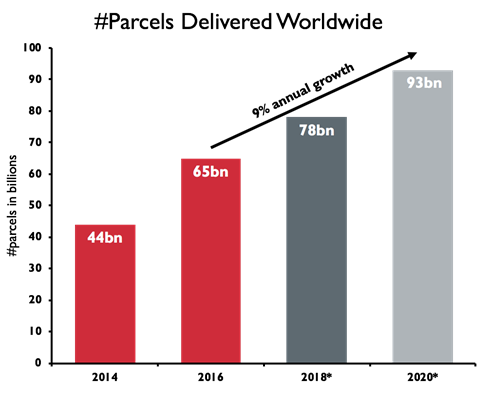
\includegraphics[width=0.5\textwidth]{images/ParcelsDel.png}\\
	\caption{Parcels Delivered worldwide [billions]}
	\label{fig:introduction__loremipsum}
\end{figure}

Responding to the increased demand of small-sized frequent shipments incurred by e-commerce has become one of the biggest challenges for logistics express delivery companies.
A successful delivery of shipments to consumers distributed across large geographical areas
will require re-designing of the existing system.

The increase of business-to-consumer (B2C) e-commerce activities implies that business are border less, global e-commerce is selling products or offer services across the world.


The idea to investigate delivery service based on the  blockchain proposed by the TU Berlin. The DC3 team in this project did not focus on implementing the blockchain system but rather in creating a platform interface to manage the parcel. At the end of the day, DC3 aims to be a part of a B2B blockchain solution that will make cross-border logistics much more reliable and efficient than they are now.   

Parcels are not always delivered at their destination in time and with the right agreed quality, this can cause financial losses due to reimbursements and low customer satisfaction. Especially higher value shipments ranging from routine parcels up to extraordinary parcels are insured against risks of loss, theft, damage or any other events that could impact delivery precision and quality. Prompt and secure detection, monitoring and recording of the shipment events is needed to allow tracking of service quality level, accountability, liability evidence in disputes and for analysis and optimization of the logistical chain.

DC3 (Dashboard for Control and Communication center) is a web-based dashboard for monitoring and controlling the logistics transactions beyond the border of a certain logistics company while leveraging DiLLaS (distributed ledger for logistics and supply chain management (DiLLaS). 

DiLLaS is an IoT and Blockchain solution that offers a new and unique view on shipment events data for logistics companies and their partners. These views create a detailed insight and transparency of significant security and safety events during the shipment. Additionally, by storing them in the distributed ledger, a trusted and decentralized recollection of the events of the shipment is created. DC3 enables a new way of handling parcel delivery and accelerates the implementation of more reliable and financial sustainable delivery processes.

The goal of DiLLaS is to provide a distributed ledger for the secure and trustworthy storage of events that occur during the transport of goods. A DiLLaS Mobile App will act as a client for the ledger and is intended as a means for all participants of a logistic chain to securely log a registration, deregistration and handover of a parcel within the distributed ledger. In combination with GRAVITY, the DiLLaS Mobile App will in addition be able to check the status of sensors that are attached to the parcels such temperature or humidity sensors and to log violations of predefined delivery conditions within the distributed ledger. Since DiLLaS makes use of Blockchain technology to persist the events and their related data in an immutable, transparent and a distributed manner where common incidents such as lost or delayed parcels can be securely traced back to its originators. With the commonly approved log of logistic events in DiLLaS, logistic operators will be able to improve their efficiency in terms of parcel delivery time by identifying bottle necks, costs per parcel by identifying unreliable partners and the quality of service by evaluating if parcels are delivered according to the predefined delivery conditions such as a constant temperature or an acceptable intensity of shocks for goods of high value. 


\section{Problem Discussion}

\subsection{Vendors communication and limitations}
There are multiple inefficiencies in cross-border delivery industry, related to lack of transparency and trust between the different logistics providers. International parcel delivery usually goes through several logistic vendors, each on their side of the border, and there is a lot of accounting and interoperability overhead in the interactions between the different vendors. The idea is to solve these issues with the blockchain technology, taking advantage of its inherent transparency and trust.
From a Logistic company perspective, the parcel information is limited to their ownership and post completion of handover to a peer logistic company the package would not be efficiently tracked and the interrelated companies handling the package would not be in consensus. This common interface provides a plausible solution to the problem stated above by giving an opportunity for the companies to keep track of the package irrespective of the ownership of the package at a given point of time by having full information about it. It will also help the companies achieve better customer satisfaction by providing such sensor options to its customers to make use of.

\subsection{Vendors HMI}
From a customer perspective, when a customer orders a parcel the information revealed to him is depended on the quality of the carrier web interface, with a unique high-detailed dashboard the customer can be independent from the retail interface system and be informed about the status of the package and location of the package at all times throughout the journey of the package from source to destination.More options are made available to the customer in terms of a temperature and a shock sensor which is capable of taking lower and upper limits from the customer as an input and reverting with any irregularities in the package.


\chapter{Related Work}
\label{cha:relatedwork}

Historically messages were usually hand-delivered using a variety of methodologies, the most common being runners and horseback riders. Then came the introduction of mechanized courier services which differed from ordinary mail services by features such as speed, security,tracking and individualization of express services. They not only started providing such services within a town or a city but started offering worldwide services. The problem being very evident with such services is tracking these packages as stated above. Such offer services are made worldwide, typically with hub and spoke model. The spoke-hub distribution paradigm is a form of transport topology optimization in which the companies organize routes as a series of "spokes" that connect the outlying points to a central "hub"[1].

These companies further utilize courier software which provide electronic proof of delivery and electronic tracking details of the package limited to ownership. Currently the gap incorporated among logistic companies on cross country deliveries are handled using basic communication or with the help of some third party companies. Eurosender is one such  company that provides a platform for businesses and individuals to have a unified solution to run their logistics processes globally. They provide services for customers ranging from a simple package delivery to Freight transport. They also help their customers track the package based on individual  tracking numbers produced by each of the logistic companies for the delivery of the packages.

Further with respect to look and feel of the application being developed, we were provided with a front-end SPA template "Crystal React Bootstrap Dashboard". Crystal React Bootstrap is a multipurpose admin dashboard created using the technologies React,Redux and Bootstrap. Its main goal is to help create complex applications using a lot of simple and easy to use React components that are embedded in this template. This template is helpful to create many kinds of dashboards relating to the health sector, online social networking websites and also for companies in need of a dashboard.

This template mainly consists of the below mentioned simple packages that could be useful for the development of an end-to-end application.

\begin{itemize}
\item Charts
\item Buttons
\item Notifications
\item Sweet Alert
\item Redux Form
\item AirBnB React Dates
\item Google Map and Uber Vector Map
\item React Bootstrap Table
\item React Big Calendar
\end{itemize}

\chapter{Concept and Design}
\label{cha:conceptanddesign}

DC3 dashboard has 3 different types of personas - Company, Customer and Postman. Hence we had to design the system differently for each user persona. Our front end application is a Single Page Application (SPA) using react JS. Our back-end is developed by using Node JS leveraging Express framework. 

\section{Architecture}
DC3 follows a modular approach for the whole system. As shown in the bigger picture, entry point for the system is social login, Google in this case. we are using passportJS which can be used to integrate other social strategies e.g. GitHub, Facebook as well. Furthermore, passport does provide local strategy as well where we can configure local database as well for authentication and authorization. This feature would be useful when we different vendors does deploy their own instances of the diLLas service and want to authorize the existing customer base from their own system. we have detailed overview for google authorization explained later as well 

\begin{figure}[!ht]
	\centering
	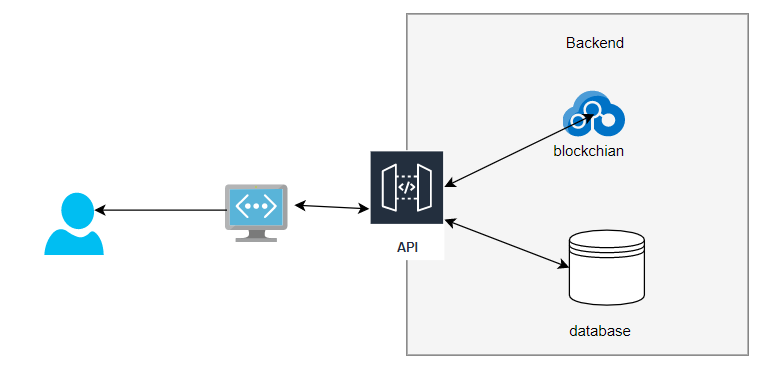
\includegraphics[width=1 \textwidth]{images/bigger_picture.png}\\
	\caption{System Architecture(abstract view)}
	\label{fig:System Architecture(abstract view)}
\end{figure}

Once user is logged-in, for example from browser, an access-token is stored into the local session storage for being used on the front end SPA (Single Page Application) react app.  This token is used for further communication between front-end and back-end. It contains user profile and authorization info. This info is leveraged to protect the different endpoints on the server side and provide related data based on the user type. For example, when a customer hits the /packages endpoint he will be able to see his own packages only but when a company user hits the same endpoint, he will get all the company level packages in the response.

\section{Authentication and Authorization with Google}

Authentication is a vital part of the project and most real world applications need authentication and authorization. While authentication identifies some entity as a valid user, authorization defines the actions that the user is allowed to perform, based on his/her roles and rights. There are many solutions to provide for authentication or authorization in an application and we had two major choices,

\begin{itemize}
\item First one was to keep user state management on Redux.
\item Second was to use a Facebook or a Google Authentication integration with our application.
\end{itemize}

We chose to go with the second choice as it was a new learning for the team to integrate it with our application using the PassportJS framework, it also reduces the burden of the users to register themselves rather directly sign in with their Google accounts and more importantly because it provides back-end services to securely authenticate users, paired with easy-to-use client SDKs. It can authenticate users using passwords and federated identity provider credentials.  

In our application, once the user clicks on the Google authenticate button,it directs the user to Google's OAuth 2.0 server, which requests access to the user's meta data from the Google drive with a read only scope. Further after granting or denying the access to the user, is then redirected to the original page, which pareses the access token from the string. The page then uses this access token to make  a simple API request which calls the Drive API's to retrieve the information about the authorized user's Google account. If this request is successful then the API response is logged in the browser.
For the first time user's we check our local database to determine the existence and add the user to our database if the user name does not exist and fill in the vital information using the above fetched information from the authorized user's Google account. We have achieved the same with the help of the PassportJS framework where it provides us local strategy to configure our local database for such authentications. Also if the user name exists before hand, we validate the token from the server side with the OAuth2.0 provider and once validated, a JSON Web Token (JWT)  is produced to securely provide authorization to the front end.
We use a main component in our database table "Persons" that is "PersonType" component which determines the role given to a user.Based on this value we determine if the user is either a customer,postman or a company representative. The role with the lowest features is the role of a user, which is the value provided by default to the user on first time log in and henceforth the company role has  authorization to upgrade the user to a postman or a company representative. Initial company role setup is done by the admin. The below figure provides a overview of the functioning of the Google authentication and Authorization based on role integrated to our DC3 application.

\begin{figure}[!ht]
	\centering
	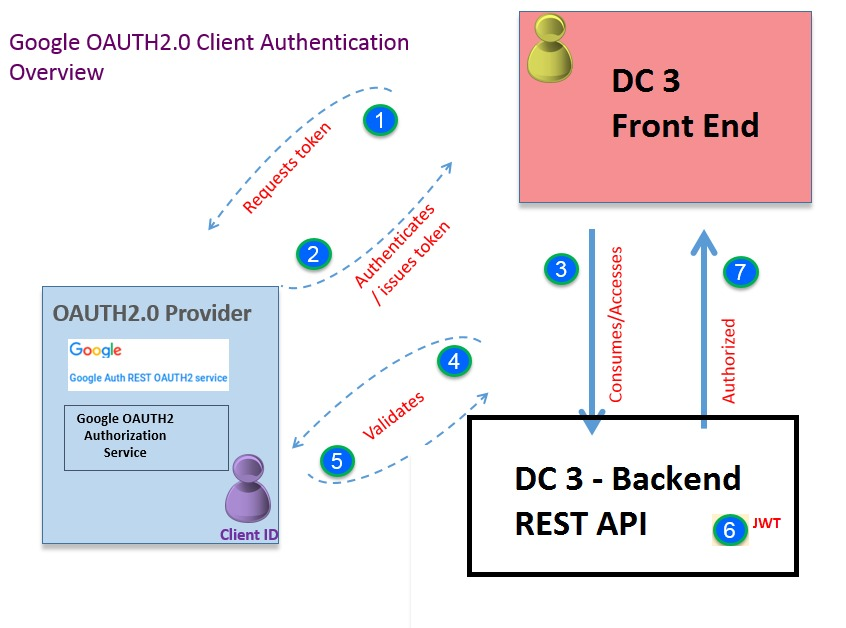
\includegraphics[width=0.5\textwidth]{images/GoogleAuth.jpeg}\\
	\caption{Authentication \& Authorization}
	\label{fig:Authentication and Authorization}
\end{figure}


\section{Database Design}
DC3 database has 8 tables. Order, Person, Order History and Order sensors are the major tables while others play an important role as well.  Designs majorly circulate around Orders table. We have normalized the database to avoid storing redundant data e.g. Order and Sensors had many to many relationship so we divided it and created another table, OrderSensors. Let’s understand the philosophy behind each table


\subsection{Company}
The company table is persisting the information about all the companies. It stores the company name and a brief description of the company. 

\begin{table}[!ht]
	%\small
	\centering
	\begin{tabular}{ |l|l|l| }
		\hline
		Id & Int - auto increment & Unique company ID \\
		\hline
		Name & varchar & Company Name \\
		\hline
		Description & varchar & Brief company description \\
		\hline
	\end{tabular}
	\caption{Company table}
\end{table}



\subsection{Address}
Address table is maintaining all kind of address across the whole system, be it order adree or customer home address. Hence it has relationship with Order and Person. Order table has two address Ids, each for pick and delivery address of the order



\begin{table}[!ht]
	%\small
	\centering
	\begin{tabular}{ |l|l|l| }
		\hline
		AddressId  & Int - Autoincrement & \\
		\hline
		StreetAddress  & varchar & \\
		\hline
		City  & varchar &\\
		\hline
		Country  & varchar &\\
		\hline
		PostCode  & int &\\
		\hline
	\end{tabular}
	\caption{Address table}
\end{table}



\subsection{Sensor}
The sensor table is a repository of unique sensors we have available in the system. It will store the names, and different possible thresholds a specific sensors has. It was designed in a generic way to store the different sensors in the same table. 




\begin{table}[!ht]
	\small
	\centering
	\begin{tabular}{ |l|l|l| }
		\hline
		Id  & Int - Autoincrement  & \\
		\hline
		Name  & varchar & \\
		\hline
		MinValue & varchar & Minimum possible reading for the sensor  \\
		\hline
		MaxValue & varchar & Maximum possible reading for the sensor\\
		\hline
		DisplayUnit  & varchar & \\
		\hline
	\end{tabular}
	\caption{Sensor table}
\end{table}


\subsection{Person}
The Person table is storing various kinds of user information. It stores personal information for the company, customer and postman. Additionally, it maintains the social login values for the user. Once a user signs up, it defaults to a customer but admin or company user can change his role to postman or admin (company) user. 

\begin{table}[!ht]
    \begin{center}
    \begin{tabular}{ |l|l|l| } 
    \hline
    Id & Int - auto increment & Unique company ID \\
    \hline
    FullName & varchar & \\
    \hline
    Email  & varchar & \\
     \hline
    Password & varchar & Minimum possible reading for the sensor \\
     \hline
    DateOfBirth & varchar & Maximum possible reading for the sensor \\
     \hline
    PersonType & varchar & Person type e.g. customer, postman or company \\
    \hline
    PersonRole & int & Stores person role or associated company id \\
    \hline
    GoogleProviderId & varchar & Google user-id \\
    \hline
    GoogleAccessToken & varchar & Logged-in user access token\\
    \hline
    \end{tabular}
    \end{center}
    \caption{Person table}
\end{table}

\subsection{Orders}
Orders table is keeping most of the data in the database and it will have a higher churn rate than any other table in the whole system. It stores a lot of referential ids from other tables than actual data e.g. pick \& drop address, person, company. It also consists of the status of the package which determines to be the major representative of package information.

\begin{table}[!ht]
\begin{center}
\begin{tabular}{ |l|l|l| } 
 \hline
Id & Int - auto increment & Unique Order ID \\
 \hline

OrderID & Int - AutoIncrement  & \\
\hline
PickAddressID & Int & Pick up address id\\
\hline
DropAddresID  & Int  & Drop address Id\\
\hline
PickDate  & date & Registration or pick up date\\
\hline
ArrivalDate & date & Delivery date\\
\hline
PersonID & int & Package Sender id\\
\hline
ReceiverPersonID & int & Package Receiver id\\
\hline
Status & varchar & E.g. Registered, In-Transit or Delivered\\
\hline
CompanyId & int & Reference for associated company\\

 \hline
\end{tabular}
\end{center}
    \caption{Orders table}
\end{table}

\subsection{OrderSensors}
OrderSensors table consists of all the vital information of the sensor be it the threshold of the shock sensors or the threshold of the temperature sensors. It also consists of the values recorded for the package and is differentiated using the combination of OrderId and the SensorId entities being considered from the above tables.
\begin{table}[!ht]
\begin{center}
\begin{tabular}{ |l|l|l| } 
 \hline
Id & Int - auto increment & Unique sensor ID \\
 \hline
OrderId & Int &  \\
 \hline
SensorOd & Int & \\
 \hline
MinThreshold & Int & Minimum Threshold for sensor\\
 \hline
MaxThreshold & Int & Maximum Threshold for sensor\\
 \hline
valuerecorded & Int & Value recorded by the sensor\\
 \hline
light & Int & Definition of light impact \\
 \hline
heavy & Int & Definition of heavy impact \\
 \hline
severe & Int & Definition of severe impact \\
 \hline
bclight & Int &  \\
 \hline
bcheavy & Int &  \\
 \hline
bcsevere & Int &  \\
 \hline
bctemprature & Int &  \\
 \hline
\end{tabular}
\end{center}
    \caption{OrderSensors table}
\end{table}

\subsection{Incident}

The Incident table consists of all incident raised by all users in the form of a unique incident Id and a brief description of the incident. It is linked with the user and the packages using the OrderId and the PersonId respectively.
\begin{table}[!ht]
\begin{center}
\begin{tabular}{ |l|l|l| } 
 \hline
IncidentId & Int - auto increment & Unique Incident ID \\
 \hline
Description & varchar & Brief Incident Description \\
 \hline
OrderId & Int &  \\
 \hline
PersonId & Int &  \\
 \hline
\end{tabular}
\end{center}
    \caption{Incident table}
\end{table}

\subsection{Database Diagram}
\begin{figure}[!ht]
	\centering
	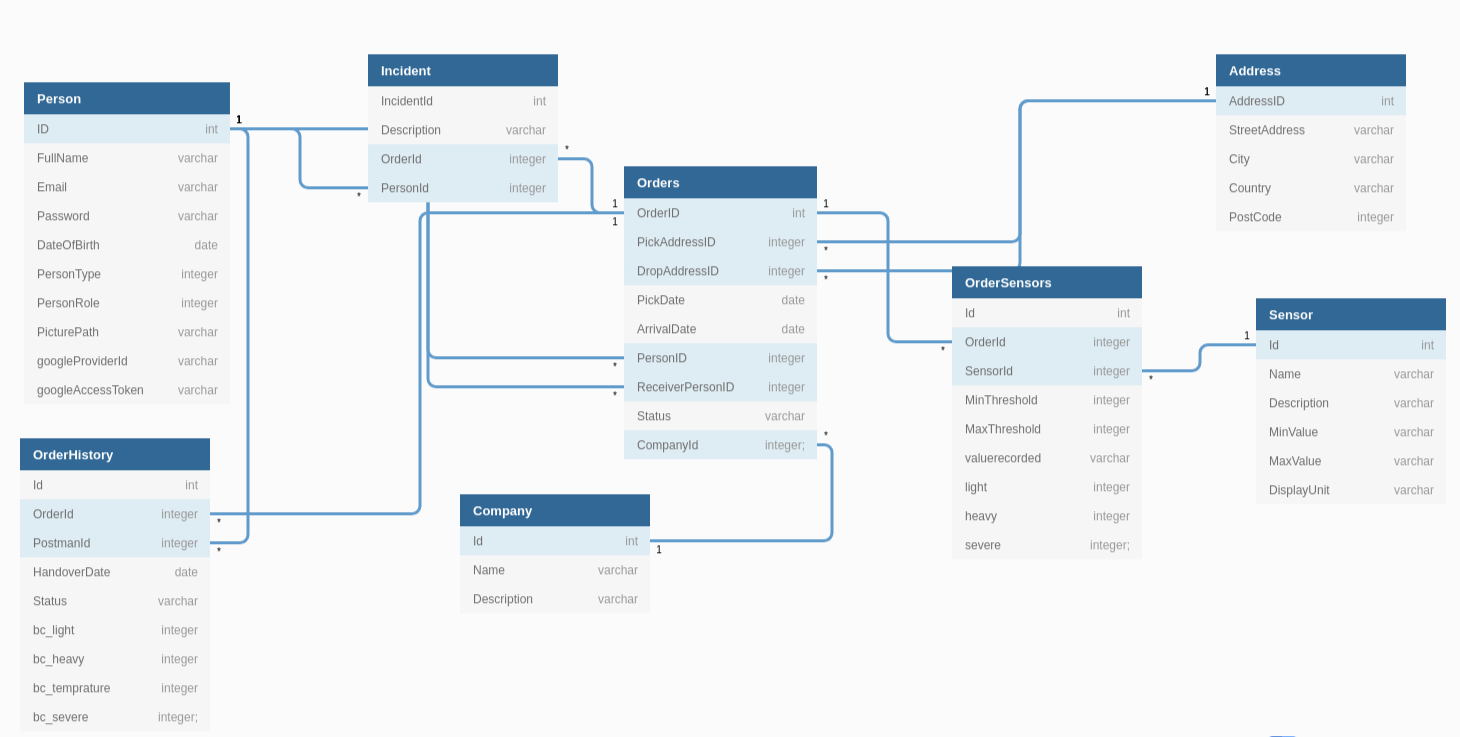
\includegraphics[width=1\textwidth]{images/IOSLDBDiagramlatex.png}\\
	\caption{Database Diagram}
	\label{fig:Database Diagram}
\end{figure}

\chapter{Project Organization}
\label{cha:projectorganization}


This chapter will cover how we organized the entire project. We will uncover the the project timeline in the first section, how roles were distributed among the members in the second section and also the major tools and infrastructure used in the final section of the chapter.
\section{Timeline}
\begin{figure}[!ht]
	\centering
	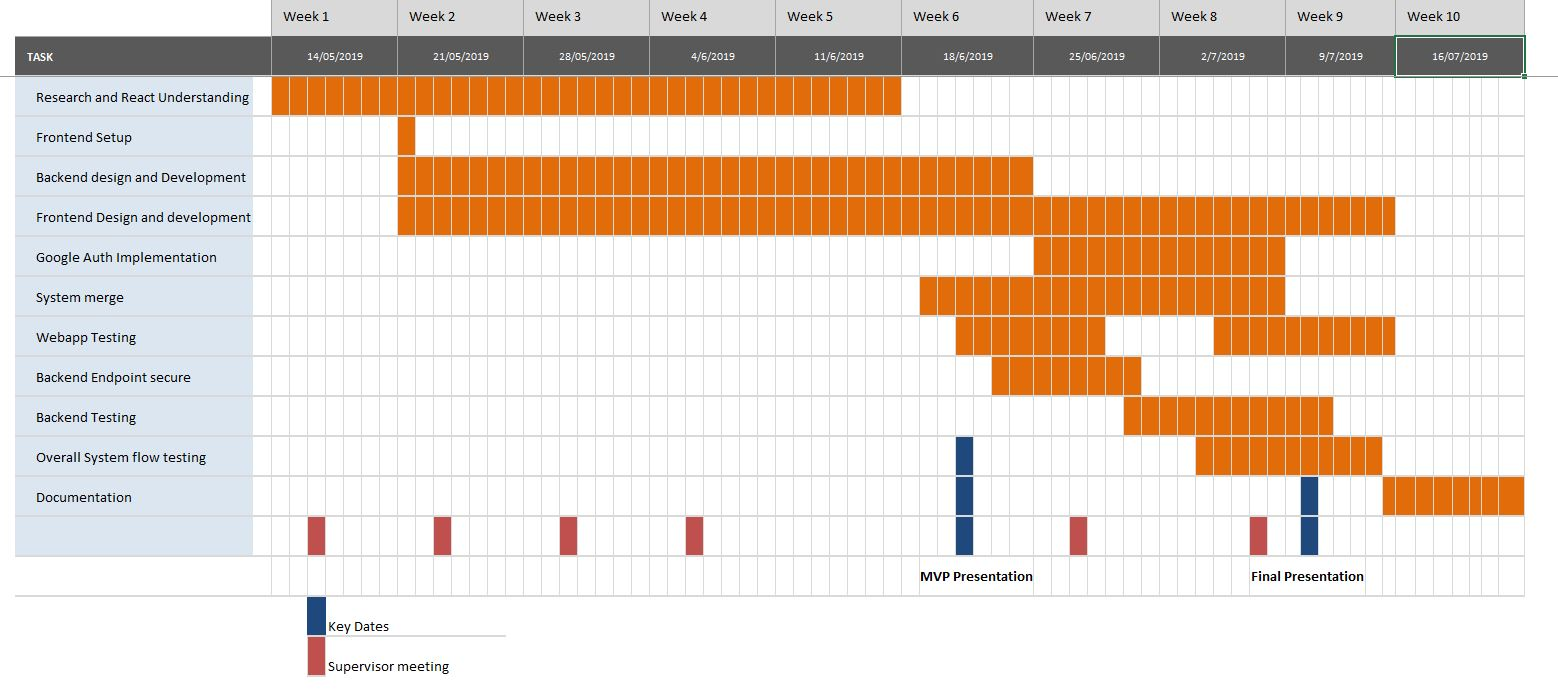
\includegraphics[width=1\textwidth]{images/Timeline.jpg}\\
	\caption{Project Timeline}
	\label{fig:Project Timeline}
\end{figure}

\section{Work Distribution}
\begin{table}[!ht]
\begin{center}
\begin{tabular}{ |l|l|l| } 
 \hline
\textbf{Task} & \textbf{Team Member} \\
 \hline
Customer & Alon \\
 \hline
Company & Kiran  \\
 \hline
 Postman & Anubhav \\
 \hline
 Integration, Routing and Common Web pages & Pradyumna \\
 \hline
 Backend & Haseeb Asif \\
 \hline
  Documentation & All Members \\
 \hline
\end{tabular}
\end{center}
    \caption{ Task Distribution }
\end{table}
To fulfill the requirements of the project in the given time span, we initially divided the task among our team members with five vital tasks and a common task of documenting the code and project as a common task for all the team members as shown in \textbf{table 4.1}.Team member responsible for his/her user space design was responsible to come up with a basic design for the web page and share it among the other team members to be in-sync with the other team members to make sure that the web pages had some consistency through out the project. Git hub was the basic source control used by our team which consisted of the master branch considered to be the actual application and other nodes created by members to work on their relevant tasks.Team member responsible for each user space had the responsibility to develop the complete functionality of the task given to them based on the requirement provided. The team member who was provided with the task of the customer persona was responsible for all customer functionality and so on a similar trend followed for the other major tasks.Integration, routing and common web pages that were common for all personas was a task which included the development of the landing page, user log in,overall routing or navigation inside the application and system integration with back-end. The back-end task which was quite elaborate the team member responsible for the same had to provide an overall database design and implement the same according to the system requirement with appropriate end points being given to the front end developers based on functionality. Documentation of the code and the project was obviously handled by all of the team members to provide inputs on all aspects of their work and the project in general.

Although the tasks are quite strictly divided based on the above task distribution table, we as a team always worked together providing ideas to each other on different tasks to make sure of the overall consistency of the application and also gain collective input and expertise of the entire team where it was necessary.
\section{Tools and Infrastructure}

\begin{itemize}
\item Github - Source control (iosl-dc3, iosl-backend)
\item Trello -Task mgmt (https://trello.com/b/RXwlgcJI/iosl-dc3)
\item Slack - Communication (https://iosltu2019.slack.com)
\item Overleaf- Documentation Collaboration (https://overleaf.com)
\item VS Code - Code editor
\item Azure for Postgres SQL - Database
\end{itemize}

\chapter{Implementation}
\label{cha:implementation}

In this chapter we explain briefly the techniques used to implement both the front-end and the back-end.
We first elaborate on the different roles existing in the front-end:

\section{Frond-end}

\textbf{IDE}: Visual Studio code\\
\textbf{Language}: React\\
\textbf{Libraries used}:
\begin{itemize}
    \item React-router-dom
    \item Receiver mail must be a registered user
\end{itemize}


\subsection{Home Page}
\textbf{http://localhost:3000/\#/}\\*
\\*
After a successful log in all roles (postmen, company, customer) will be redirected to the same home page.
This home page presents a table containing a minimized version of the package data as per the role.
The user can here get a brieg=f information regarding the packages under his/her ID and its corresponding status.\\*
Algorithm:
\begin{enumerate}
    \item Extracting the user role. Each user as part of the Google authentication has a role type stored in the local database upon first time log in.(postman, customer, company) 
    \item \textbf{http://localhost:8000/packages/user/}  get request, before the component is mounted : upload package and information. The information will then be displayed as a table.
\end{enumerate}



\subsection{customer}
Libraries used:
\begin{itemize}
\item rc-slider - for creating the temperature slide bar 
\item react-horizontal-timeline - for the time line view
\item redux-form - for the registration form
\end{itemize}

The customer role refers to any individual who sends a package through the system.
The customer has the following abilities:

\begin{itemize}
    \item Register a package
    \item Delete a package
    \item view a package detail  
    \item view time line of the package
\end{itemize}


\subsubsection{Register a package}
\textbf{http://localhost:3000/##/packages/registerPackage}\\
\\*
The register package process is divided into two components:
\begin{itemize}
\item RegisterPackage.js - view 
\item UserSpace.js - controller 
\end{itemize}


\begin{figure}[!ht]
	\centering
	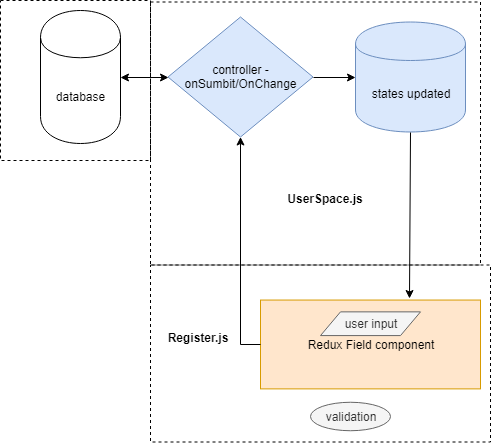
\includegraphics[width=0.5\textwidth]{images/register.jpg}
	\caption{register package process, component diagram}
	\label{fig:}
\end{figure}


The component RegisterPackage is an assembly of Redux <Field> component and React input.
for each input field the user enters, the specific page is rendered and the consequent state is updated.
The form contain the following validation:
\begin{itemize}
\item No text input field can be left empty 
\item Receiver mail must be a registered user
\end{itemize}
i.e without standing in the form requirement, the user can not press the submit button.

When registering a package, a sensor data may be provided by clicking on the corresponding check box. It is important to mention that not every package needs to have sensor data.\\*
Algorithm:
\begin{enumerate}
  \item \textbf{http://localhost:8000/address} post request,enters the address and returns an ID for each address provided.
    \begin{enumerate}
        \item \textbf {http://localhost:8000/packages}  post request, enters the package to the packages table, returns a package ID procided an address ID as input
        \begin{enumerate}
        \item \textbf {http://localhost:8000/OrderSensors}  post request, enters the sensor information (if exists)  into the sensors table, returns a sensor ID provided a package ID as input
        \end{enumerate}
    \item \textbf {http://localhost:8000/OrderHistory}  post request, enters the action(registration) as part of the order history to be used later on as part of the time line display - If and only if a package and sensor id is provided\\
    \end{enumerate}
\end{enumerate}

Only after fetching the data successfull from the database the page content will be replaced to a "package has been registered" message.


\subsubsection{Cancel package}
\textbf{http://localhost:3000/#/packages/active}\\

The feature cancel package allows the user to cancel a package.
After pressing the navigation bar with the "delete package" option, the user will be directed to the Active.js component.\newline
The user will be shown a data-minimized table only with packages in a "registered" status, \textbf{any other package which has been dispatched already cannot be canceled}.\newline
From the system perspective while the package is being canceled, the data is not deleted from storage,it will only be marked as canceled.\\*
Algorithm:
\begin{enumerate}
  \item \textbf{http://localhost:8000/packages/user/}  get request, before component is mounted : upload all packages with "registered" status,
  \item If user deletes a pacakge:
  \begin{enumerate}
      \item \textbf {http://localhost:8000/packages/:id}  put request. Change the specific package to "canceled" status.
      \item \textbf {http://localhost:8000/OrderHistory}  post request. Update the time line, add an event to Orderhistory table.
\end{enumerate}
\end{enumerate}


\subsubsection{Detailed package view}
\textbf{http://localhost:3000/##/package/ID}\\
\\*
The feature allows the user to view extensively the package information and the package time line.
After choosing the specific package ID in the home page,the user will be redirected/routed to this component.This ID will be transfer ed as a property from the home page to the Detailed.js component. 
In addition to the package data which was provided during the registration, the table also displays the current status of the package and the condition of the package.i.e if the user requests for a sensor, the table will display the number of events where the condition was not satisfied.
The sensor data will be only present if the user registers a sensor to the package.\\*
Algorithm:
\begin{enumerate}
  \item \textbf{http://localhost:8000/packages/details/id}  get request, before component is mounted : uploads the package information. The information will be displayed in the form of a table
  \item \textbf{http://localhost:8000/packages/orderHistory/id}  get request, before component is mounted : uploads the package history.The history willthen be sent to the Timeline.js component as a property.
  \begin{enumerate}
      \item Timeline.js uses the npm package "react-horizontal-timeline" to display the package in the form of a time line.
      the time line displays the status of the package, the company and postman name related to the package at that instance.
    \end{enumerate}
\end{enumerate}


\subsection{Company}

Company user in the system will be able to do the following activities:-

\begin{itemize}
\item \textbf{View package pickup request sent by customer to the particular company.}
When customer registers package, package is registered to DC3 database with registered status. Company will see assigned package on the system filtered by status.
\item \textbf{Accept package pickup request from customer my assigning to the postman under the company.}
The registered package is accepted by company by assigning to available postman of the company for pickup from the customer location. Company does this by clicking Assign button which calls assign.js. Company has to enter the email address of postman on the form and click the button. After the package is assigned to particular postman the status of package will be change to Transit in the database. There is Assign Package Sub-menu under User Management for the package assign function
\item \textbf{Upgrade users to postman or another company user of the same company.}
Company can upgrade registered user to postman or to another company user of the same company by entering email address. For the upgrade function to be applied to particular user. The user has to register themselves as customer first. There is sub menu on sidebar under User Management for this function. UpgradeUser.js is used for this functionality.
\item \textbf{View tracking history of packages under the company.}
When company user login to the system, in the dashboard there will be all the list of packages that have been under the particular company. By clicking on order ID on the leftmost side it takes to detail page of particular company with tracking history of the packages shown as timeline.
\item \textbf{View user list of own company and change their role to available roles in the system.}
Company can see user list of and upgrade individual to postman or another company user as discussed above.
\item \textbf{Create incident for the packages}
Company can create incident for the particular packages if any alteration on the condition is noticed. For this purpose a separate menu is established on sidebar as Incident Management. Incident are created by putting Package ID and incident description under Create Incident sub-menu. 
\item \textbf{View and resolve the incident of particular packages.}
Company can view and resolve the incident for packages if those incident has been resolved. For this company has to click resolve incident button on the incident list displayed in Incidents sub-menu under Incident Management menu.
\end{itemize}


\subsection{Postman}

\begin{figure}[htp]
    \centering
    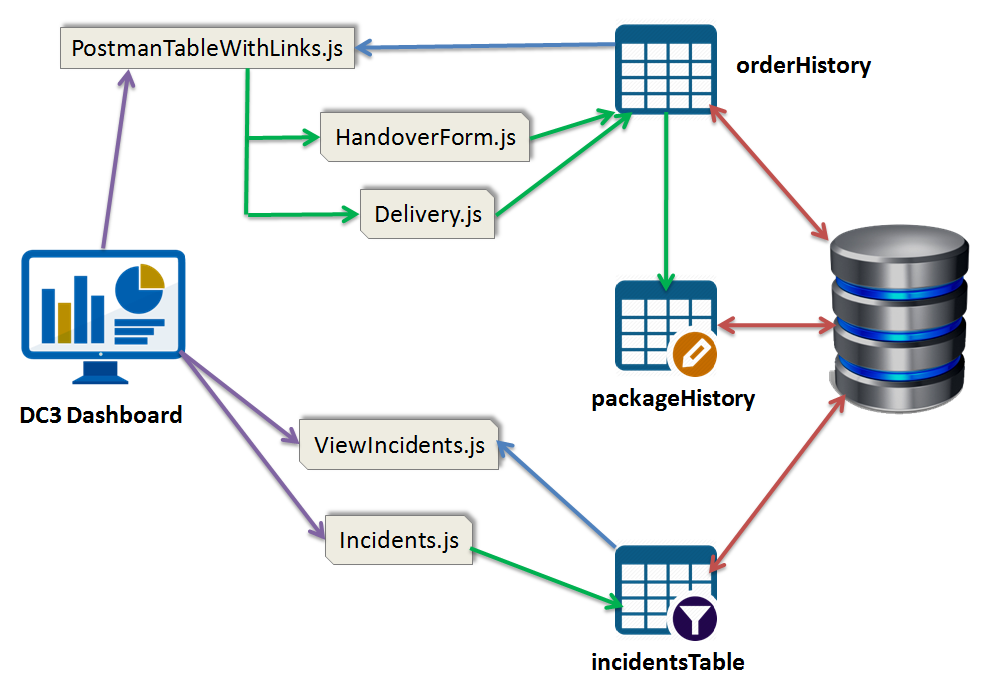
\includegraphics[width=4 cm]{images/snet/DC3 Postman.png}
    \caption{DC3 Postman}
    \label{fig:}
\end{figure}

\textbf{Overview of the functionality:}

Postman user in the system will be able to do the following activities:-
\begin{itemize}
\item {\textbf{View all the packages that have been assigned to him: }}(PostmanTableWithLinks.js) When the Company user assigns a package (PackageId) to a particular postman (PostmanId) then a relevant record is created into the table orderHistory. All the packages that are assigned to the current user are fetched using http://localhost:8000/orderHistory

\item \textbf{View the information about the package such as pickup address, drop address, status etc:} The table orderHistory contains columns that hold the relevant data of the package required for the postman to identify every package.
\item \textbf{Able to change the status of the package as Delivered once the actual delivery has been made:} whenever a postman physically delivers the package to the recipient at the respective Drop Address, then he is able to press the button 'Deliver' that invokes the function to setthe status of the Package as 'Delivered' and enter a new row in the packageHistory table only to denote that the package is now counted as one of the delivered packages.
\item \textbf{Able to Handover the package by assigning it to another Postman and change the status accordingly: }whenever a postman reaches an intermediate point in the route of the package where he has to hand it over to another postman, then the 'Handover' button is used to redirect to another component HandoverForm.js where the user id of the receiving postman needs to be entered. This functionality allows one postman to assign a package to nother postman by changing the 'AssignedTo' data in the relevant table. After this subroutine is invoked the handed over parcel  starts to appear in the dashboard of the receiving postman.
\item \textbf{Able to raise Incident whenever there is any violation of policies:} A postman to who the package has been assigned or handed over is able to judge the condition of the package and raise an incident mentioning the details of the package and the nature of violation also mentioning its current condition using the form created in the Incident.js component.
\item \textbf{View the Incidents that have been raised in the past: }Under the heading 'Incident Management' there is a link 'View Incidents' that redirects to ViewIncidents.js component that pulls data from the Incidents table and allows the Postman to see the relevant list of Incidents raised by or against him that have not yet been resolved.
\end{itemize}


\subsection{Integration, Routing and Common web pages }

\subsubsection{Integration}
As per the aforementioned statements in the earlier section, we have developed a Single Page Application (SPA) which holds together or integrates our complete application. In the application we render only one main page with a constant navigation bar and a side bar which provides usage features present on the navigation bar and the side bar based on authorization with respect to the role being assigned to the user.
The main page is further made of the header component, the footer component and the main component. The header component contains mainly the navigation bar which includes brand logo and a common sign out option for all users and the footer component contains a common footer that is rendered at all times in the page.
Further the main component inside the main page consists of the side bar and the user information.This component is rendered always as part of the SPA.The user information is itself a smaller component that displays the name, type of customer and a display picture of the user. The side bar consists of options that differ for each user based on the role assigned to the user. The main challenge here was to render the specific options with respect to role and all the common options that needed to be available for all the users in common.

The navigation bar and the side bar in our application is developed using the Bootstrap framework. It contains the duo of React and Bootstrap.The "NavBar" component was primarily used to develop the navigation bar and the side bar. Many features to toggle between entities or collapsing based on conditions were made use of from the "react-bootstrap" library with the help of some components like "Nav", "NavItem", "NavDropdown", "FormGroup", "FormControl" which were made use for better structuring of web page.

\textbf{Libraries used}:
\begin{itemize}
    \item react-bootstrap
    \item react-redux
\end{itemize}

\subsubsection{Routing}

Having our application as a single page application, it is vital to route through to correct pages or render correct components on click of routing links or buttons.
Having said that, all of our routing in the application takes place by clicking on options being rendered on the side bar or the navigation bar. As mentioned in the previous section authorization based rendering of features were first done post this on click of an option we routed the exact path of the component which was to be rendered upon clicking the link or the button. By using this mechanism we made sure a single main page was rendered upon log in and routed to respective components based on the specified routes.

To achieve this feature comprehensively, we used the "Route", "Router" and "withRouter" components from the library "react-router-dom" where we specified the exact path of the component by using the "Route exact path" or "Route path" features from the above mentioned components. Using these components from the libraries not only made the routing precise but also helped us to keep the code organized and well structured.

\textbf{Libraries used}:
\begin{itemize}
    \item react-router-dom
    \item react-redux
\end{itemize}

\subsubsection{Common web pages}
DC3 web application has three main roles or personas and each of which have different features provided in the application based on the type of role the user is assigned to. But some features in the applications are common for all of the users. For these features rather than developing repetitive pieces of code to provide the same, we developed a single component for the feature and reused the component as per requirement. 
The landing page is a common web page that all the users irrespective of the role can access. Apart from that the major functionality like the home page or the default page post log in is  common for the three kind of users was developed once and reused in different parts of the application where it portrays package history information on a minimized scale. It is filtered based on most recent and to a limited number of packages being displayed in a table format.

Another functionality that was common upon log in for all users was the incident management section. In the application, be it a customer, a company representative or a postman , all of them need to have authorization to create an incident with respect to a package. hence a set of common components like "create incident" , "view incident" was developed that could be reused.
On click of the "create incident" , the web page displays the incidents raised by the user with respect to the customer,  displays the incidents raised by the postman and the packages assigned to the postman with respect to the postman role and finally displays all incidents of packages that have been assigned to the specific company with respect to a company user.

\begin{enumerate}
  \item \textbf{http://localhost:8000/Incidents}  get request helps to retrieve the specific incidents with respect to the user based on roles.
  \item \textbf{http://localhost:8000/Incidents} put request helps to add an incident to the Incident table.
  \item \textbf{http://localhost:8000/Incidents} update request helps to resolve the incident by changing the status of the incident in the Incident table and will not be retrieved through a get request post status change.
\end{enumerate}

The component RaiseIncident is has a combination of "Redux" component, built using a "form" component.
for each input field the user enters, the specific page is rendered and the consequent state is updated.
The form contains the following validation:
\begin{itemize}
\item No text input field can be left empty,
\end{itemize}
which clearly notifies that without standing in the form requirement, the user can not press the create incident button to submit the form.

\textbf{Libraries used}:
\begin{itemize}
    \item react-router-dom
    \item react-redux
\end{itemize}


\section{Back-end}
Back-end or server is a layer on top of the database and Blockchain for the front-end. It does handle the authentication and authorization and does take care of fetching and sending data to the hyper-ledger fabric. We are using following technologies 

\textbf{IDE}: Visual Studio code\\
\textbf{Language}: JavaScript\\
\textbf{Frameworks}: NodeJS with Express



\subsection{Project Structure}
Project structure has is modular and functionality has been divided into folder based on functionality. Hence we have two major folders at the root, server and test, with some other application level files 


\begin{figure}[htp]
    \centering
    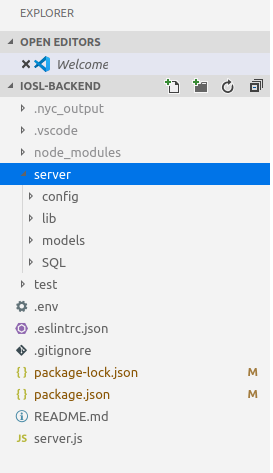
\includegraphics[width=4cm]{images/directystructure.png}
    \caption{Directory Structure}
    \label{fig:}
\end{figure}

\begin{itemize}

\item {\textbf{Server}}: This folder contains all the logic related to server functionality. 
\begin{itemize}
\item {\textbf{Config}}: This folder contains the configuration for the server side. authkeys.js does contain the secret keys used across the application for google social login and to generate the token for authorization. Passport.js contains the logic for google strategy. we can write another strategy in the same file as well e.g. github or local strategy. In future, When we are going to integreate the platform with different vendors, we will be using the local passport strategy using the vendor database. After that, route.js does contain all the routes for the application. any new routes needs to be registered in this file. Finally token.util.js contains utility functions to generate and send the token to the client back. It also exposes the method to generate the token which is used for mocked unit testing. 

\item {\textbf{lib}}: Library or lib folder does contain the middleware for our back-end application. Right now we have only one, secureMiddleware, to secure our API endpoints. It does check if access-token header is provided in rquest body, cookie or querystring and then decode it using our secret. If successful it will set the user profile on the request object, otherwise throw 401 response. 

\item {\textbf{models}}: Models folder does contain all the different models to fetch the data from database or block chain. Each file represent an entity in the system or a related database relation.  Furthermore, index.js file contains the references of all the models and is used almost everywhere in the system as single reference point for the models. 

\item {\textbf{SQL}}: SQL folder contains the database schema which can be used to deploy or create the database while setting up a project on a new machine. Additionally, it contains a schema file to generate the database diagram on dbdiagram.io as well. 
\end{itemize}


\item {\textbf{test}}: This folder contains all the unit tests. Each file contains the tests for the respective model file. Test does use mocha and chai frameworks.

\item {\textbf{env}}: .env is environment file to setup variables at the start of the project instead of reading from the config file, it will be read from the environment. This file is git ignored. It isn't used at the moment as we are reading db config from the db.js directly for now. 

\item {\textbf{eslintrc.json}}: ESlint configuration can be changed using this file. We are using Airbnb base syntax for our linting.  

\item {\textbf{gitignore}}: GitIgnore is used to tell git which files we don't want to store in the source control. 


\item {\textbf{package.json}}: This file contains all the configuration to setup the project. When we do npm install, it will read this file and install all the package on end user machine. It also contains the dev dependencies. We have different scripts configured to run e.g. running the server or run server in the debug mode, run linter. 

\item {\textbf{server.js}}: This is the starting file where our project starts. This file will bootstrap the application by configuring different modules, followed by loading the routes and then running the http server on specific ports. We also configure the express server, body parser (which parse the request body), cookie-parser, passport js and most importantly CORS to send cross origin requests.   

\end{itemize}

\subsection{Unit Testing}
We are using mocha framework for unit and integration testing in our project. Additionally we have used chai as an assertion framework for our tests. Each test has a title or test case description followed by request and expected results. A sample test is as follows

\begin{verbatim}
  /*
  * /GET company/id
  * Test the single company records from the database
  */
  it('It should GET single company', (done) => {
    chai.request(server)
      .get('/company/2')
      .end((err, res) => {
        res.should.have.status(200);
        res.body.should.be.a('array');
        res.body.length.should.be.eql(1);
        done();
      });
  });



\end{verbatim}

We used chai request to call the endpoint, set the access token for the secured endpoints, and then compare the results with  the expectation. We also have tests which will send different access token to validate the authorization of the endpoints e.g. postman can see only packages assigned to him and not all the packages or a customer cannot request a handover for a package. 

\chapter{Evaluation}
\label{cha:evaluation}

DC3 web application visualizes logistic processes from blockchain data and IOT sensor monitors. DC3 system puts customers in the loop with regard to package status merging and displaying relevant information from blockchain, the local database and the IOT sensors. From registering the package to delivering the package at the final destination, customer does not have to look for different vendors and tracking options. Fully informed package condition and the exact custody holder of package can be managed by the customer using the DC3 system.
\section{System Flow Evaluation}
For the evaluation of the developed system we created separate emails (Gmail accounts) for each user. Created two for company users, two for customers and four for postman. Postman were divided among two companies for handover and delivery processes to be shown. We started from adding users to the system and registering the package into the system to delivering the registered package through the companies postman to the destination.

As there is no specific procedure on system to add user as company directly, first companies were added as customers and later changed their roles to company representatives where in reality the admin role creates the master company account and later additions can be made. And similarly a postman and a customer were added in system using Google authentication. Also postmen are initially registered to the system as customers and can later be upgraded to a postman by company users. And company can upgrade a user to a company user for its company.

For the flow of delivery of package and how that information will be displayed on system we started with the registration of a package from the customer filling in all the details required. Customer then has to assign a company from the listed companies as their initial package handler. Also the receiver has to be registered in the DC3 system for the sender to send the package to the receiver. Customer can also choose available sensors from the system that should be attached to the package to check the condition and safety of package (which is optional). For now DC3 has two sensor types to be selected among one being the heat Sensor and the other is the shock sensor. User can select either of these two or can select both sensors or even neither of the sensors.Customer has a time limit until the package is sent into the status of in-transit to actually de-register the package from the system.

Customer registered packages are displayed to the company account, where company can further assign the package to a postman belonging to the company for pickup and handover processes. For the package to assigned to a postman by the company, the package should have a registered status. The Company can then assign the package to postman by entering the registered email address of the postman.

Postman sees the list of available jobs under the account and starts to deliver packages to the receivers, hands over the package to another postman of same company or hands over the package to another postman of a different company based on the destination address. For a delivery to be complete, the postman has to deliver the package to the destination address and mark the package as delivered. And for any handovers the postman will have to enter the email address of the other designated postman and update the package details.
In between the delivery process incident creation is a function where users( company, postman and customers) can create an incident with respect to a specific package issue(s). Customer can report to the company if the package has arrived distorted, broken or in unacceptable condition. Postman can generate an incident if the handed over package is broken, torn, distorted or in unacceptable condition and company can generate an incident if they notice unusual condition on packages under their custody. The raised incident are displayed to postman, company and customer linked with the package.

Resolve incident provides mechanism to solve issues and resolve created incidents in the individual user level. Company, postman and even user can resolve created incidents if they are satisfied with the action taken by the concerned parties to mitigate the raised issues.

Each package detail displays the detailed information of the package with its time line. Time line helps to visualize the package status and also helps to determine ownership of the package at a given instance.

\section{System Limitation and Recommendation}
DC3  web application has covered all stakeholders ( customer, Postal Companies and Postman) within the system and the basic flow of the system has included all these stakeholders inside the package delivery loop. But there are some limitations in system which are as follows

\begin{itemize}
\item By using Google authentication, system cant directly detect the user type. Like for instance if a company representative wants to register in the system first they have to register as a customer and then have to manually upgrade themselves as the company user by getting in touch with the master company user.This condition also applies for postmen but it is a valid procedure.
\end{itemize}
\begin{itemize}
\item DC3 currently does not have a mechanism to fetch data directly from blockchain as the set up is not complete with respect to the blockchain ledger. Which means IOT triggered incidents are not working in the system and only user created incidents are stored in the system database for now and are displayed in the Incident management system.
\item DC3 web application is only tested in the local environment, on local PCs and laptops. No real time testing and stress testing is done for real business scenarios.
\end{itemize}
\begin{itemize}
\item Coding standards can be improved a bit generally in the front end and as all of our team members were beginners when it came to react JS development. Many of the functionality and layouts were reused/modified from the provided template hence structuring of the code is not exactly up to the industry standards. Code cleaning was done extensively but there still exists a few redundant pieces of code. 
\end{itemize}
Even with these limitations DC3 provides most of the functionality that were proposed in the requirement phase.This system can be used as a  basic product which can be improved to make it an industry standard end-to-end web application. As part of the future work the Blockchain integration can be looked upon as the major addition to the system.

\chapter{Conclusion}
\label{cha:conclusion}

Primarily a brief explanation stating the requirement was provided to the team which basically was to create a dashboard for monitoring logistics data.
The purpose of DC3 as a web application is to bring together three different user groups so that they could use a single application to monitor logistics. As per the requirements it was clear to is that the web application is supposedly used by three major user groups and hence we decided to go on and create three personas for our project.The primary focus was to create a web based application with a look and feel that matches that of the template provided to us and make sure all the functionality is to be included in the application. Post understanding the basic frameworks necessary to develop the application, we dived into the development process.The involvement of a Back-end in our case is to give completeness to the website by providing a Database for saving the user information, history of registered/delivered packages and saving incidents that occur in the middle of transit.Then came the development phase where we  actually had plenty of hit and trials; adding and removal of components; re-designing old components; adjusting the size or placement of these components on the dashboard. Also the division of work based on personas also made sure that each user group has a different view of the dashboard whist keeping a consistent outlook with the SPA approach. Further the React JavaScript being popular for its component based development actually made things more convenient to embrace the hit and trial approach of work because it made us obligated to stick on to the component based development which made the code more re-usable and also allowed us to immediately view our changes in the running local servers. In the DC3 application the presence of a NavBar component provides a rigid classification of different components to our application; for instance "Register.js" component is kept under the Package Management category and "Incident.js" is kept under Incident Management category which ensures that not all components are refreshed or in this case re-rendered while navigating from one functional component to another. When we consider the blockchain setup, ideally most of the data is to be derived by the DC3 application comes from a dedicated blockchain that constantly provides the data related to the current condition of a package and part of this data are sent by the temperature and pressure sensors allocated to a package as per customer request. This step is to be taken care of as part of the future work as the blockchain set up is yet to be completed. With inclusion of the same, the DC3 when compared to the traditional tracking services provided by the Logistic companies, gives a much more broader view of tracking and monitoring with advanced functionality that can also serve multiple logistic companies simultaneously. Considering a bigger picture, DC3 outsmarts the classical approach of logistics monitoring by providing to the users as well as the companies at the same time; It is a single platform that is capable of displaying information of registered packages that are handled by more than one company during its transit across the continent.
Finally with the diversity among our team members coming from different areas of expertise, it was not an easy task to immediately start off with the project development. We needed a few weeks to introduce ourselves to React JS platform and once familiar started developing. we were very glad as this turned out to be a huge learning curve for all the team members in terms of front end development and project management skills.We also learned as a team the importance of teamwork, regular brainstorming, collective research sessions in developing an application on the whole.Also regular meetings with our supervisor did help us a great deal to set weekly targets to be achieved in terms of the project completion. Having these smaller targets set on weekly basis kept us motivated and helped complete the project in time.Overall the knowledge and experience gained from this project can indeed be very helpful to all of us in pursuing a career in the Information Technology sector. 


%--------------------------------------------------------------
% TABLES, FIGURES, BIBLOGRAPHY AND APPENDICES
%--------------------------------------------------------------
\backmatter

% Lists of tables and figures
\listoftables
\listoffigures

% Bibliography
%\setwidesite{}						% Set page to be wider for bibliography
%\markboth{Bibliography}{bibliography}
%\label{cha:bibliography}
%\bibliographystyle{IEEEtran}
%\bibliography{bibliography.bib}

% Use following to separate online (websites) and offline (books, papers) sources
%\printbibliography[heading=offline,filter=offline]
%\printbibliography[heading=online,filter=online]

\begin{appendices}
	\chapter{Appendix 1}
\label{appendix:listing1}

\begin{figure}[htp]
    \centering
    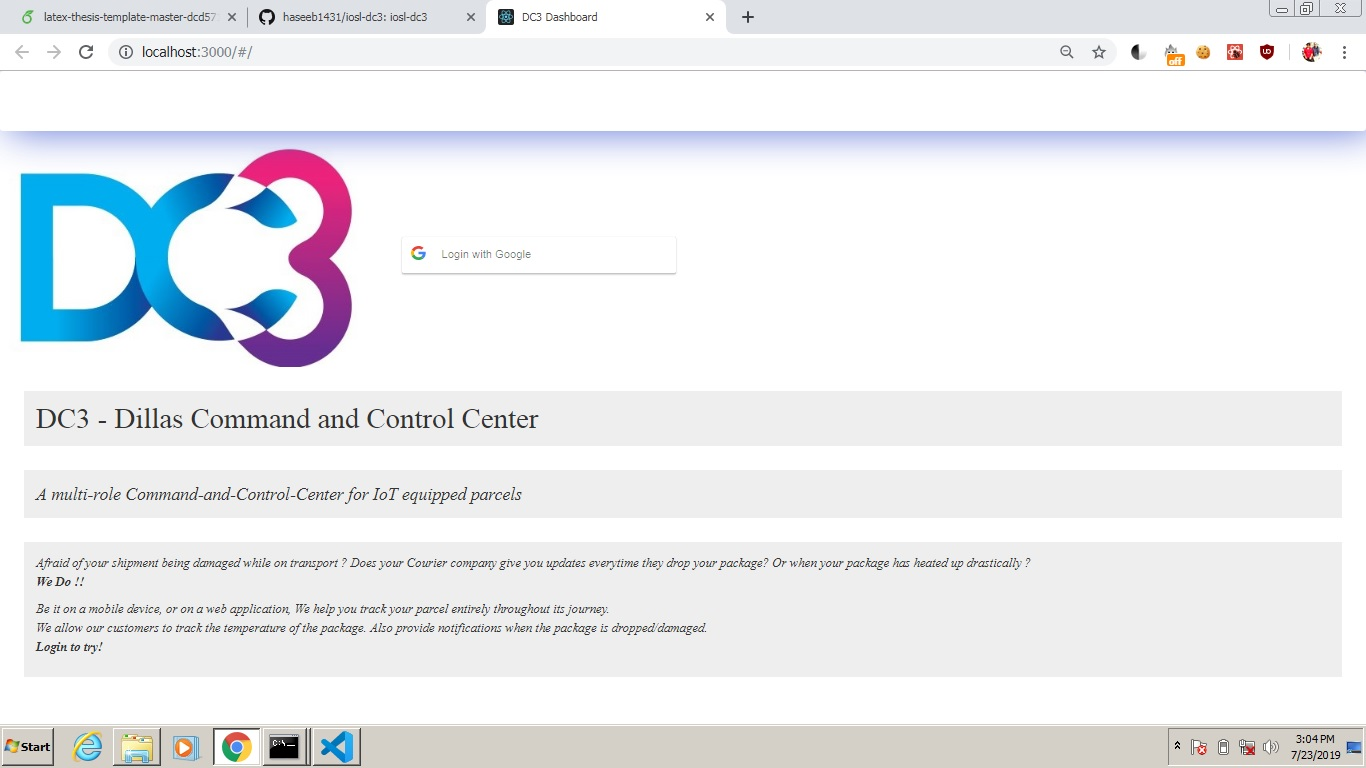
\includegraphics[width=6cm]{images/screenshots/Home.jpg}
    \caption{DC3 Landing Page}
    \label{fig:}
\end{figure}

\begin{figure}[htp]
    \centering
    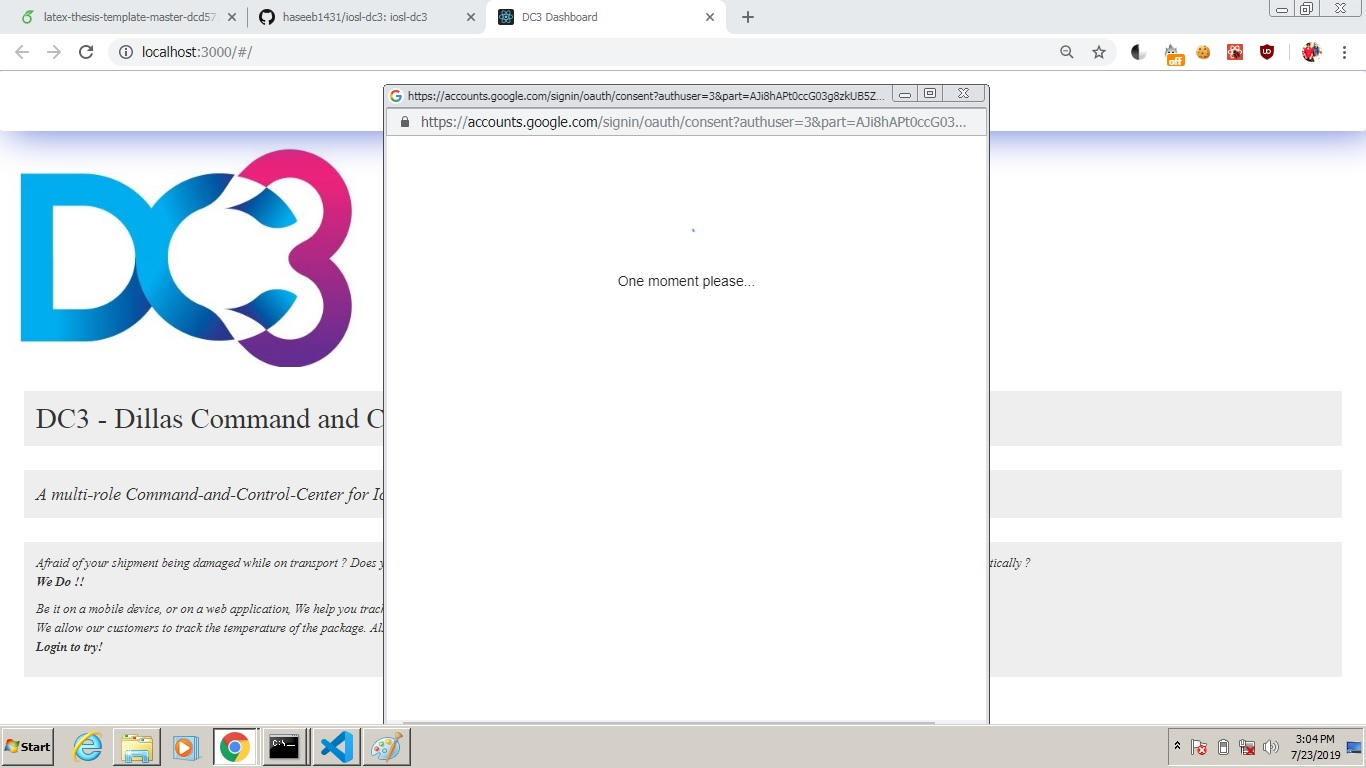
\includegraphics[width=6cm]{images/screenshots/Login.jpg}
    \caption{DC3 Login}
    \label{fig:}
\end{figure}

\begin{figure}[htp]
    \centering
    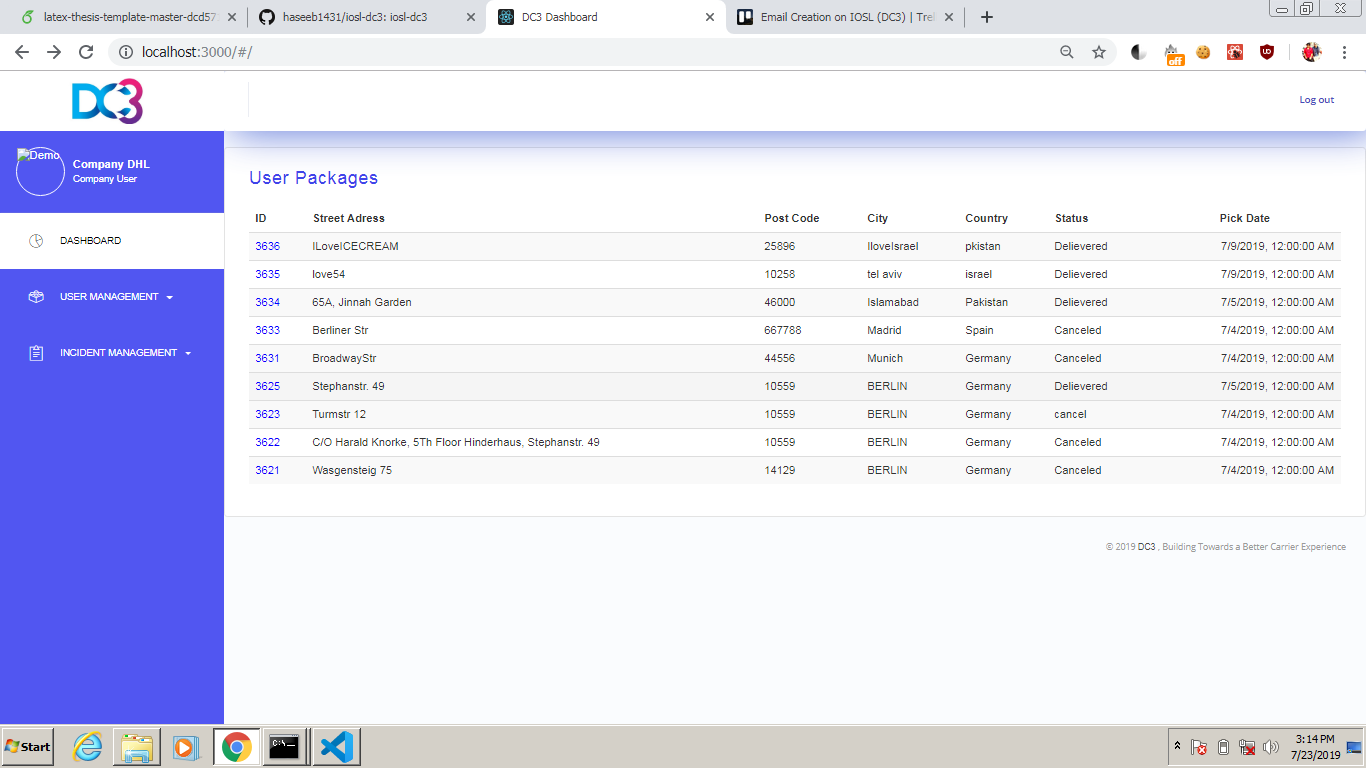
\includegraphics[width=6cm]{images/screenshots/Company_Dashboard.png}
    \caption{DC3 Company Dashboard}
    \label{fig:}
\end{figure}

\begin{figure}[htp]
    \centering
    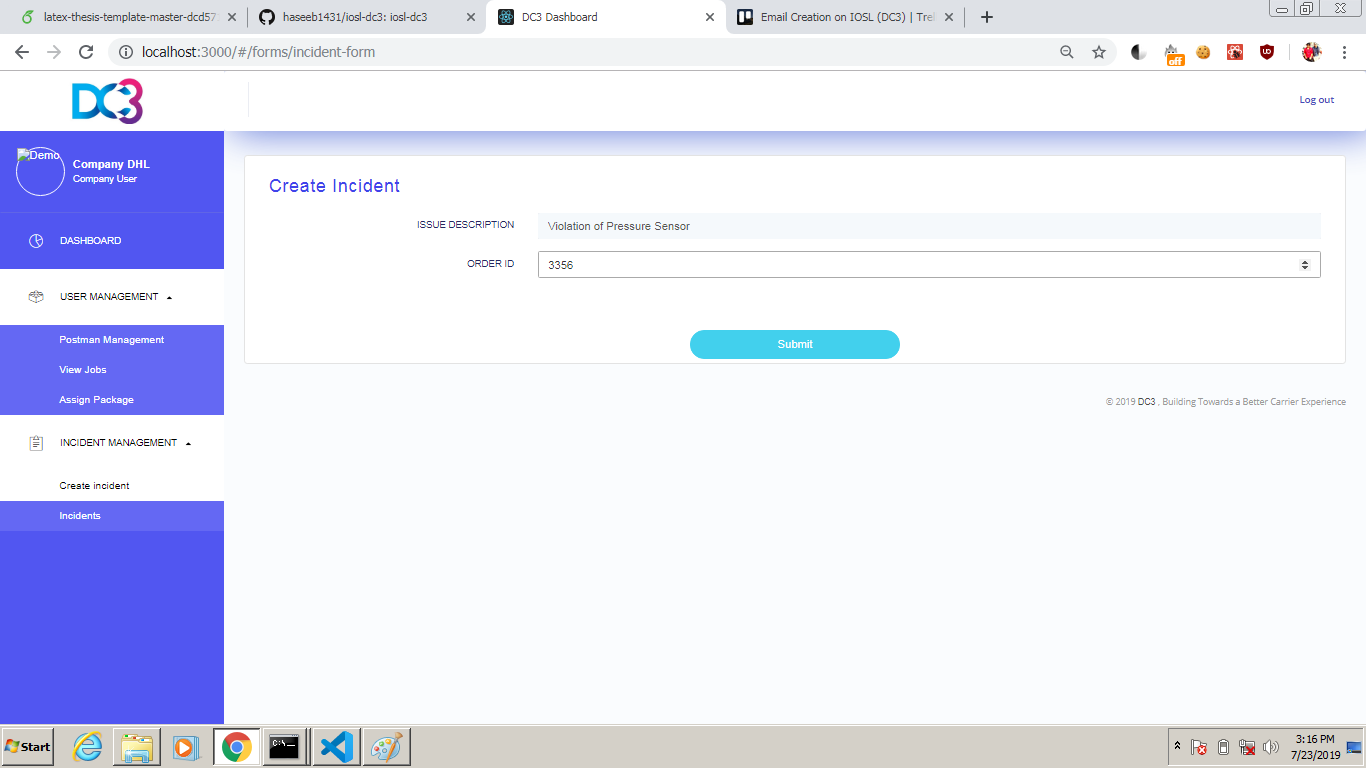
\includegraphics[width=6cm]{images/screenshots/Company_Raise_Incident.png}
    \caption{DC3 Company Raise Incident}
    \label{fig:}
\end{figure}

\begin{figure}[htp]
    \centering
    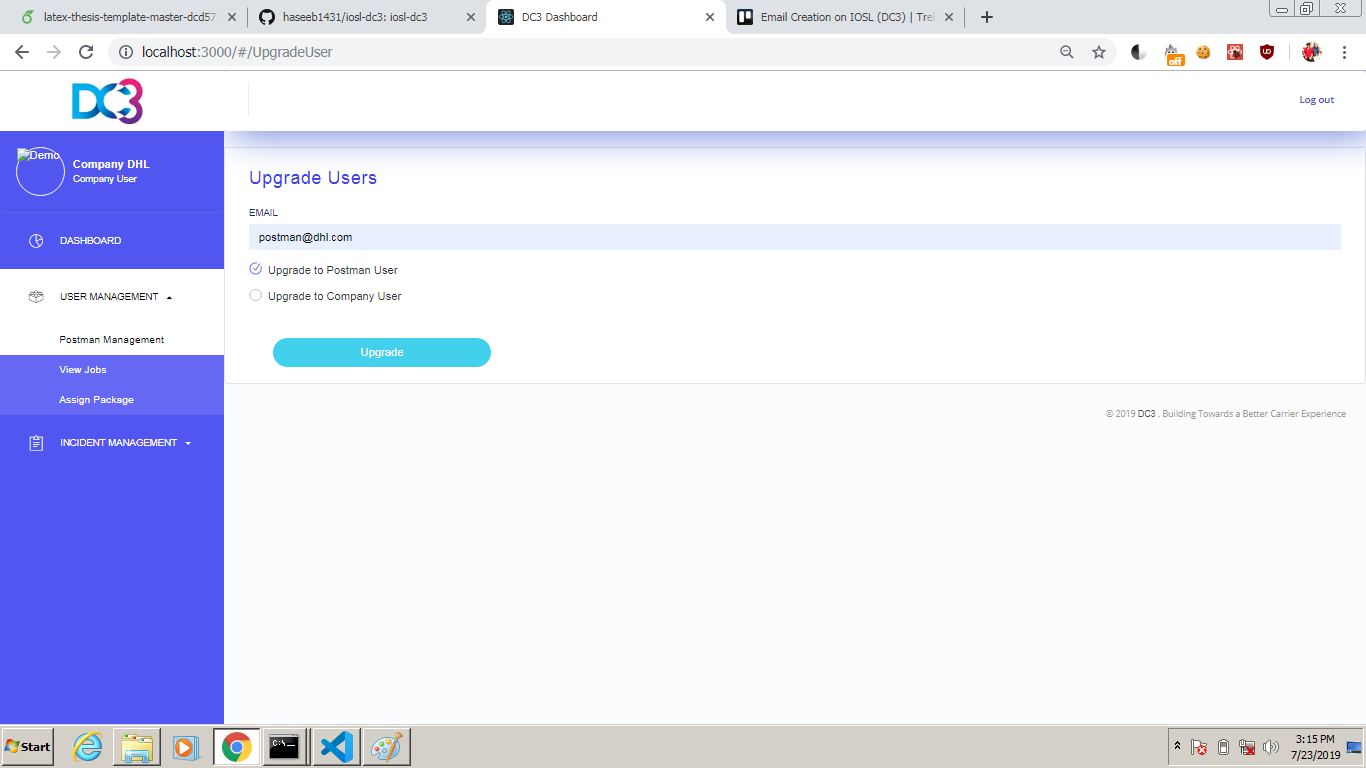
\includegraphics[width=6cm]{images/screenshots/Company_User_Mgmt.png}    \caption{DC3 Company User Management}
    \label{fig:}
\end{figure}

\begin{figure}[htp]
    \centering
    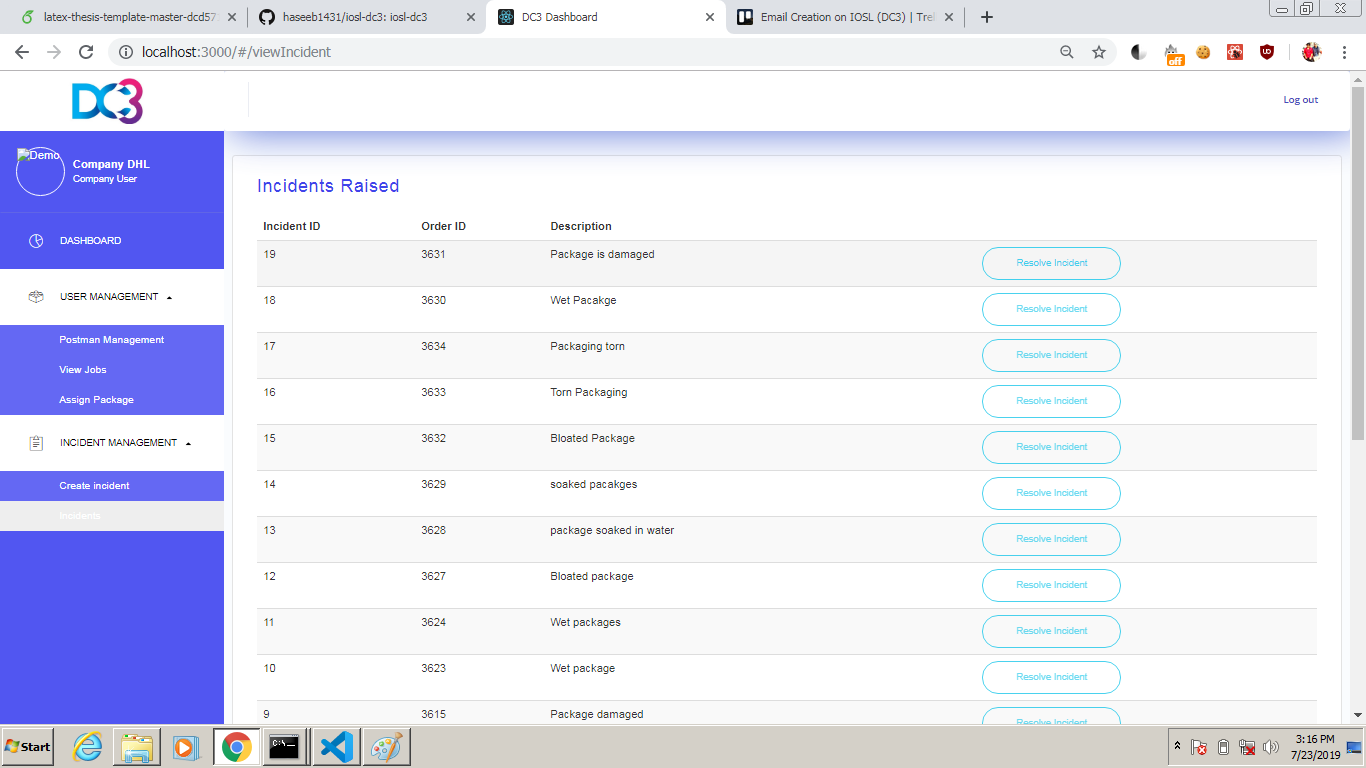
\includegraphics[width=6cm]{images/screenshots/Company_View_Incidents.png}
    \caption{DC3 Company View Incidents}
    \label{fig:}
\end{figure}

\begin{figure}[htp]
    \centering
    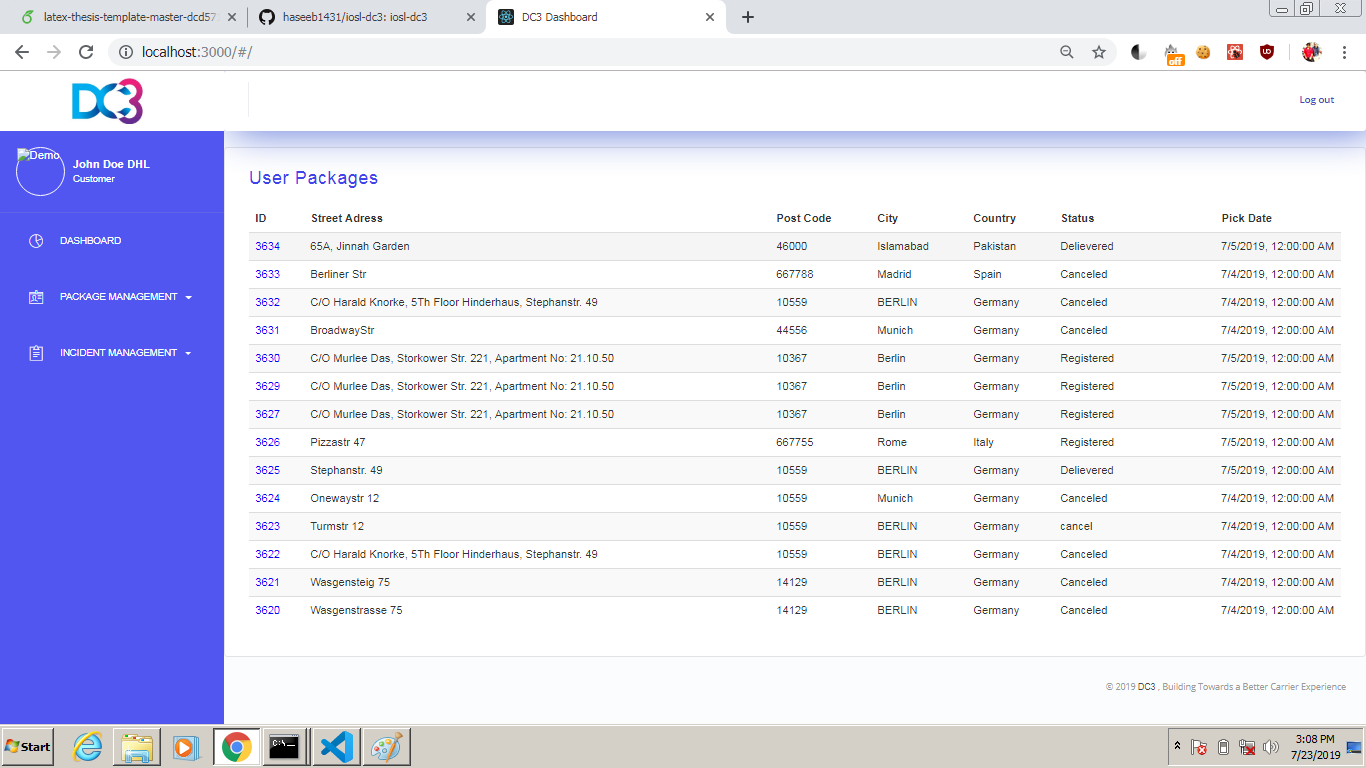
\includegraphics[width=6cm]{images/screenshots/Customer_Dashboard.png}
    \caption{DC3 Customer Dashboard}
    \label{fig:}
\end{figure}

\begin{figure}[htp]
    \centering
    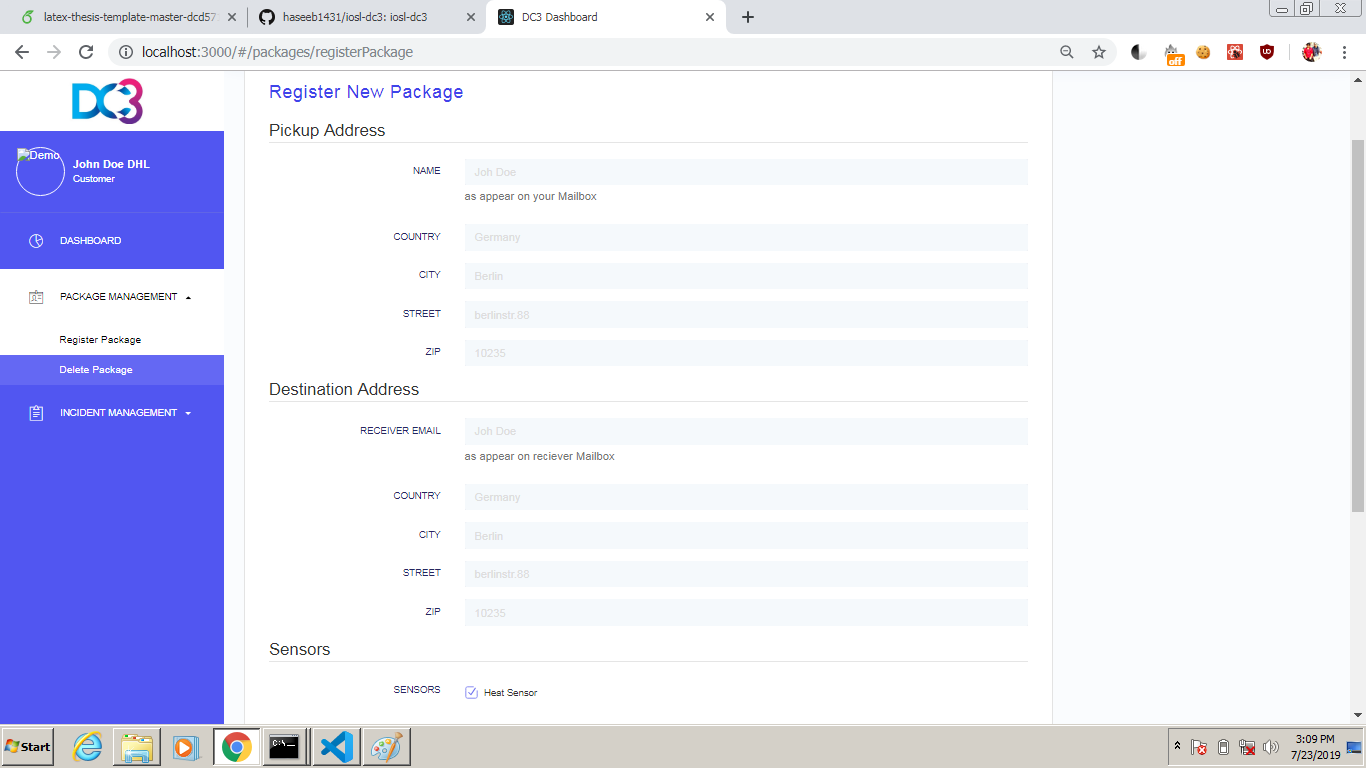
\includegraphics[width=6cm]{images/screenshots/Customer_Register_Package.png}
    \caption{DC3 Customer Register Package}
    \label{fig:}
\end{figure}

\begin{figure}[htp]
    \centering
    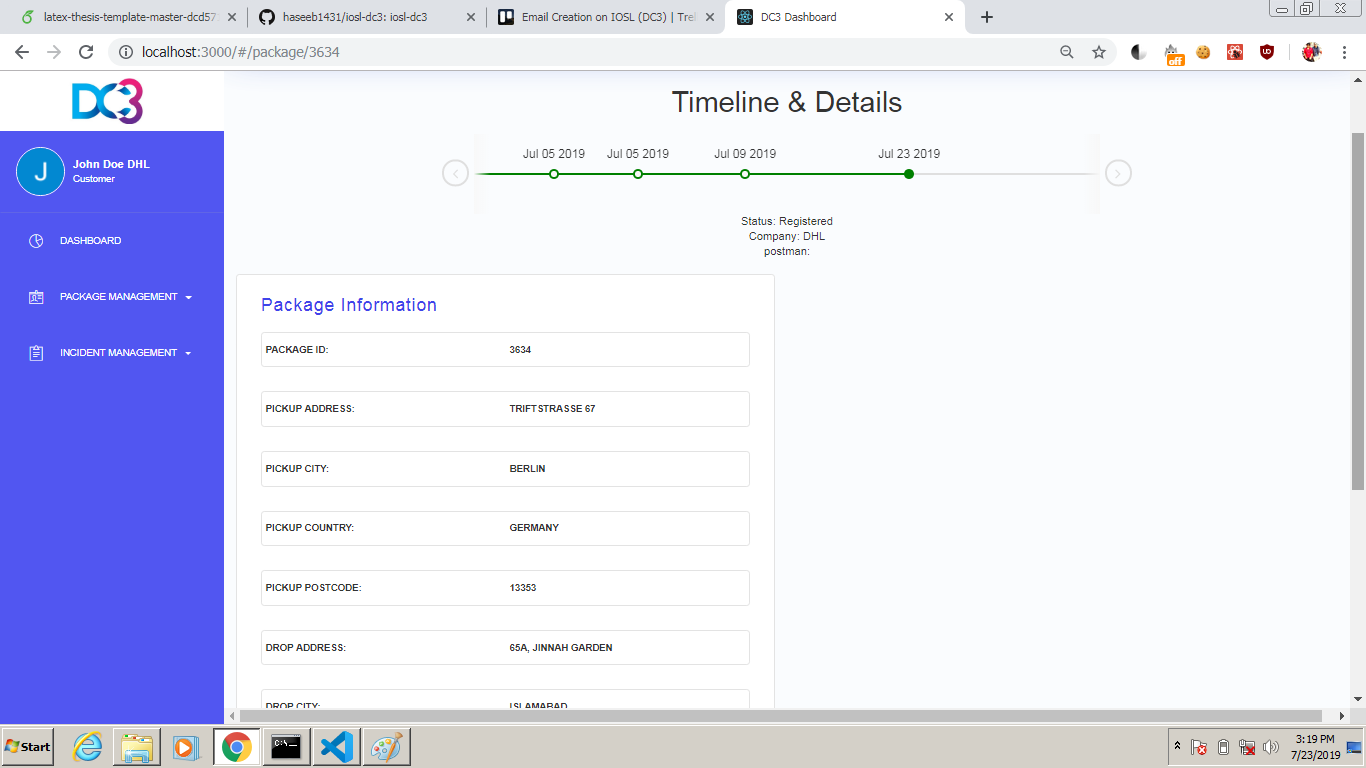
\includegraphics[width=6cm]{images/screenshots/Customer_Package_Details.png}
    \caption{DC3 Customer Package Details}
    \label{fig:}
\end{figure}


\begin{figure}[htp]
    \centering
    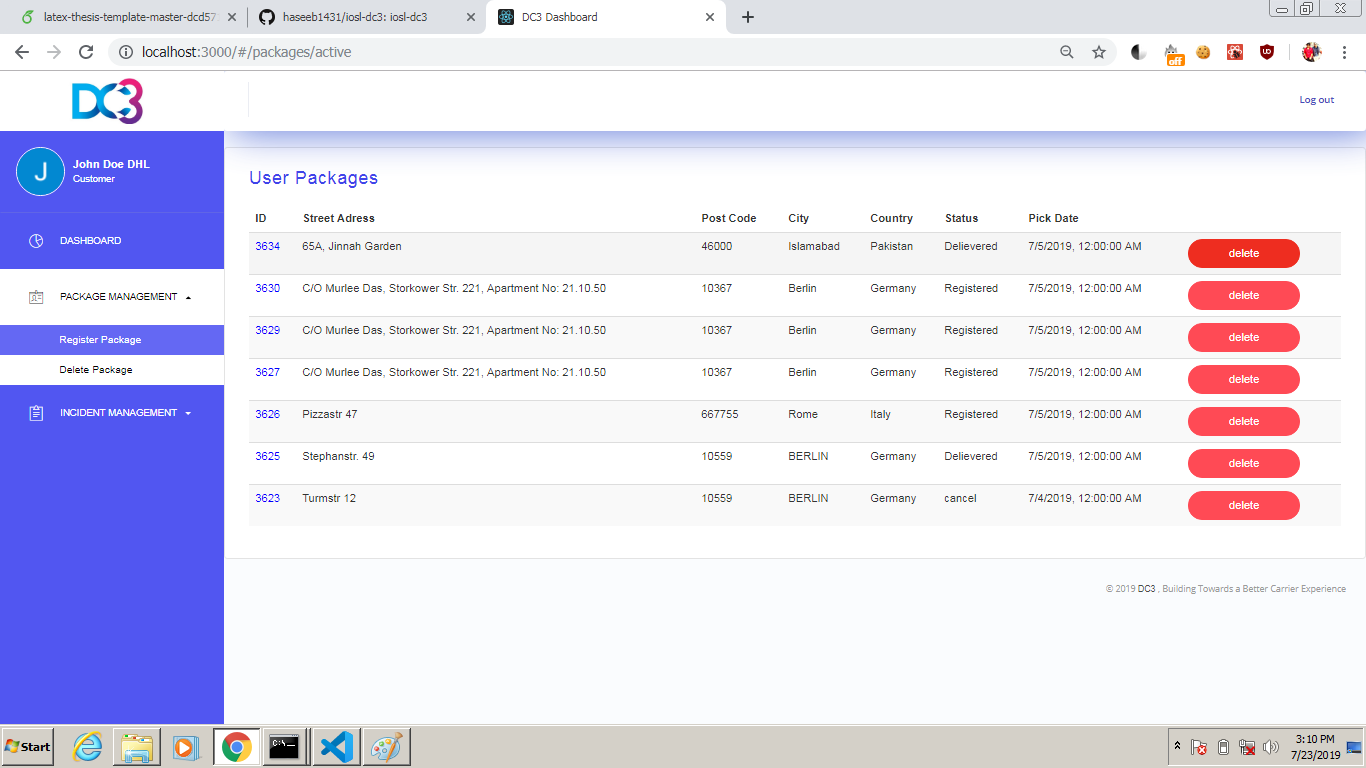
\includegraphics[width=6cm]{images/screenshots/Customer_Delete_Package.png}
    \caption{DC3 Customer Delete Package}
    \label{fig:}
\end{figure}

\begin{figure}[htp]
    \centering
    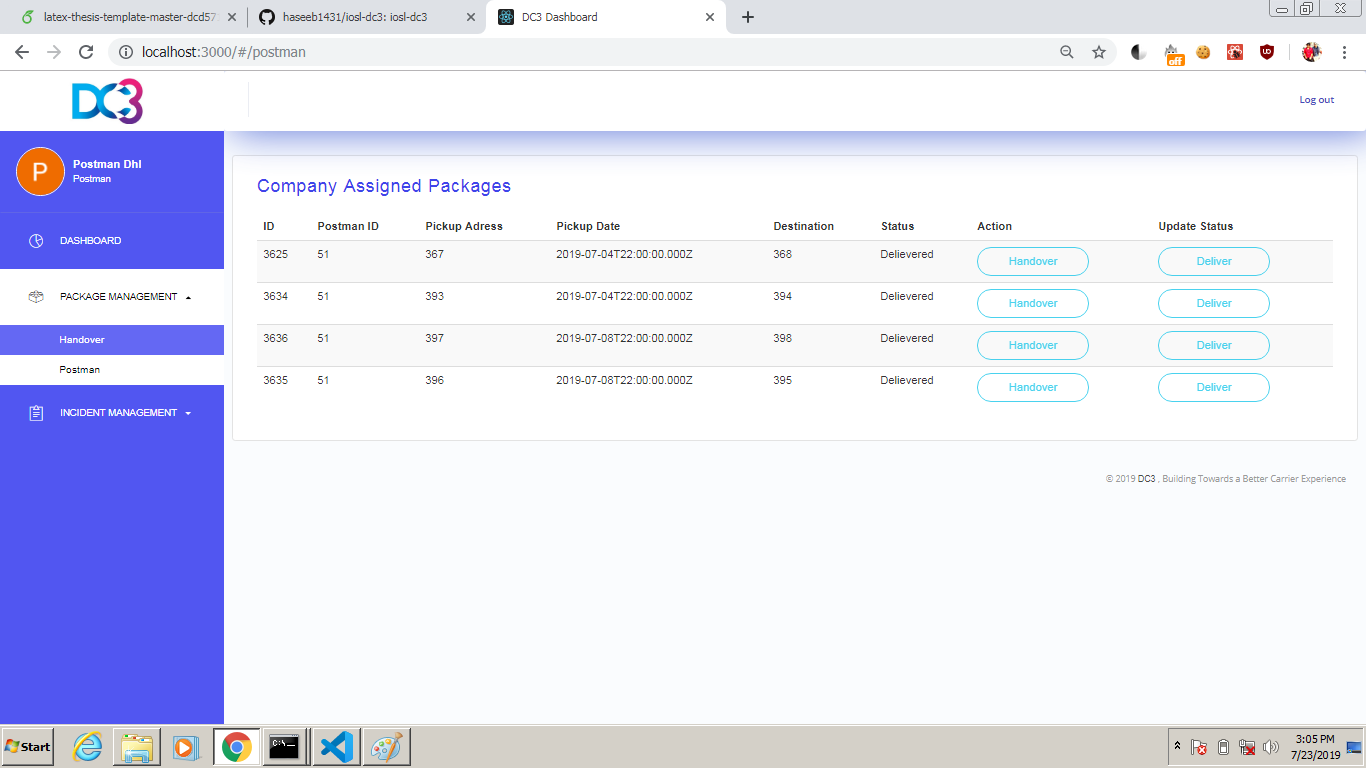
\includegraphics[width=6cm]{images/screenshots/Postman_Dashboard.png}
    \caption{DC3 Customer Postman Dashboard}
    \label{fig:}
\end{figure}

\begin{figure}[htp]
    \centering
    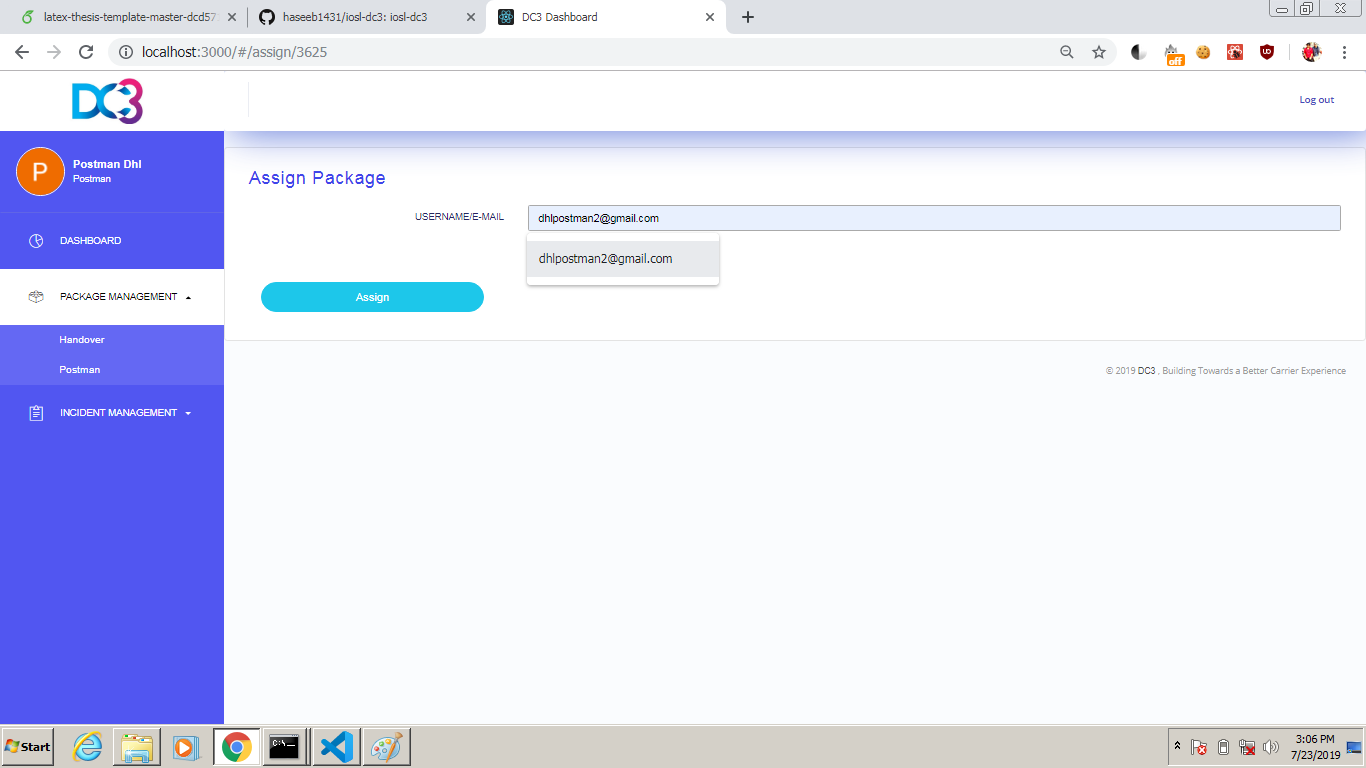
\includegraphics[width=4cm]{images/screenshots/Postman_Handover.png}
    \caption{DC3 Customer Postman Handover Package}
    \label{fig:}
\end{figure}

\begin{figure}[htp]
    \centering
    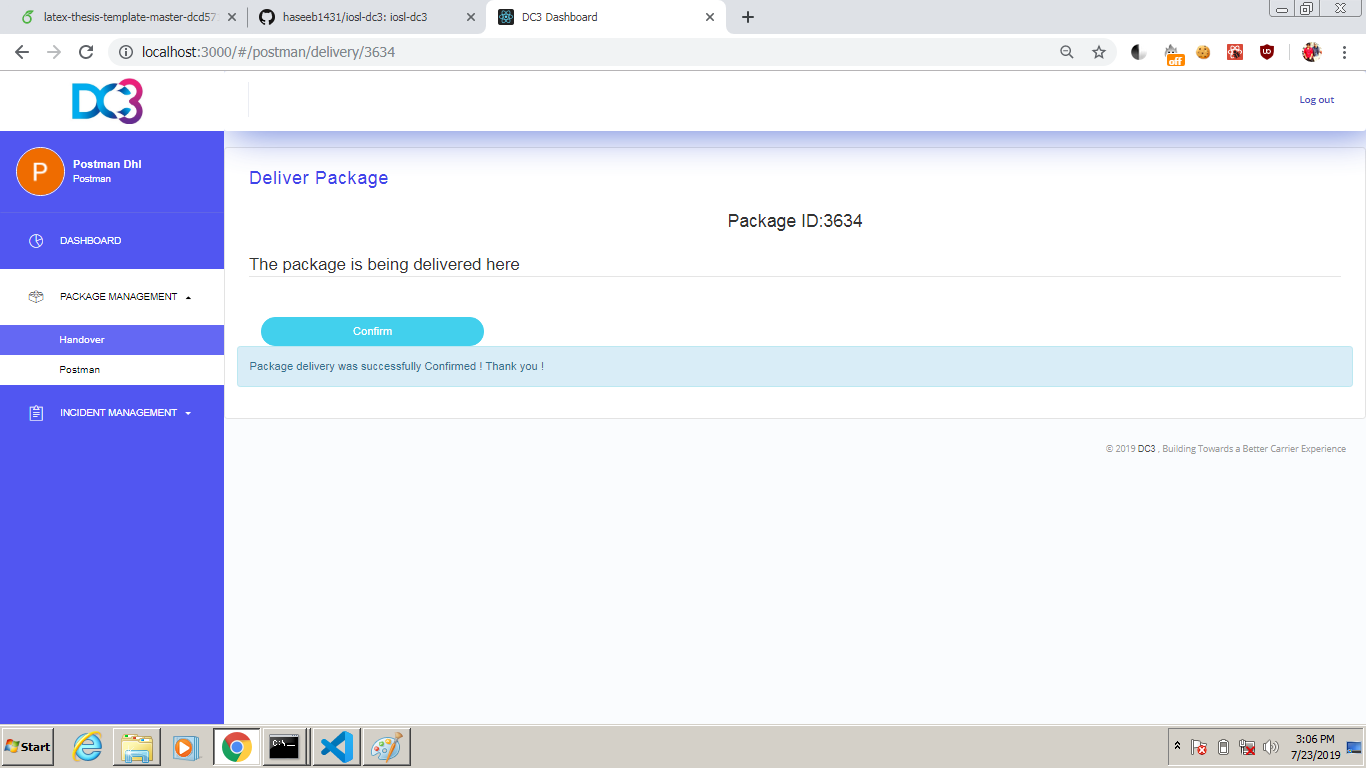
\includegraphics[width=4cm]{images/screenshots/Postman_Delivery.png}
    \caption{DC3 Customer Postman Deliver Package}
    \label{fig:}
\end{figure}


	% \input{content/99_appendices/a02_listings}
	% \input{content/99_appendices/a03_listings}
\end{appendices}

\end{document}
